%preamble\vect{\psi}_i^{T}\vect{K\psi}_j = 0\vect{\psi}_i^{T}\vect{K\psi}_j = 0
%https://www.overleaf.com/learn/latex/How_to_Write_a_Thesis_in_LaTeX_(Part_4):_Bibliographies_with_BibLaTeX
\documentclass[12pt,twoside]{report}
\usepackage[a4paper,width=150mm,top=25mm,bottom=25mm,bindingoffset=6mm]{geometry}

\usepackage{polski}
\usepackage[utf8]{inputenc}
\usepackage[T1]{fontenc}
\usepackage[polish]{babel}
\usepackage[autostyle]{csquotes} 

\usepackage[svgnames,table]{xcolor}
\usepackage{amsfonts}

%\usepackage{layouts}
\DeclareUnicodeCharacter{2208}{$\epsilon$}
\DeclareUnicodeCharacter{0229}{ę}
\DeclareUnicodeCharacter{2264}{$\ge$}
\DeclareUnicodeCharacter{0327}{?????}
%\DeclareUnicodeCharacter{0322}{!!!!!}

%BIBLIOGRAFIA
%\usepackage[backend=biber,style=authoryear,url=false]{biblatex}
\usepackage[backend=biber,style=numeric-comp,sorting=none,url=true]{biblatex}
\addbibresource{2020_08_19_My_Collection.bib}
\AtBeginBibliography{\small}

%NAGLOWEK I STOPKA
%\pagestyle{headings}
\usepackage{fancyhdr}
\pagestyle{fancy}
\fancyhf{}
\fancyhead[ro]{\slshape\nouppercase{\rightmark}}
\fancyhead[le]{\slshape\nouppercase{\leftmark}}
\fancyfoot[CE,CO]{\thepage}

%OBRAZKI
\usepackage{pgfplots}
\usepackage{graphicx}
\graphicspath{ {./figures/} }
\usepackage{caption}
\captionsetup[figure]{font=small}
\captionsetup[table]{font=small}
\usepackage[export]{adjustbox}
\usepackage{subfig}
\usepackage{float}
\newsavebox{\measurebox}


%wzory
\usepackage{amsmath,bm}
\usepackage{mathtools}
\usepackage{scalefnt}


\newcommand\ScaleExists[1]{\vcenter{\hbox{\scalefont{#1}$\exists$}}}
\DeclareMathOperator*\bigexists{%
	\vphantom\sum
	\mathchoice{\ScaleExists{1.5}}{\ScaleExists{1.4}}{\ScaleExists{1}}{\ScaleExists{0.75}}}
\newcommand\ScaleForall[1]{\vcenter{\hbox{\scalefont{#1}$\forall$}}}
\DeclareMathOperator*\bigforall{%
	\vphantom\sum
	\mathchoice{\ScaleForall{1.5}}{\ScaleForall{1.4}}{\ScaleForall{1}}{\ScaleForall{0.75}}}


%lista
\usepackage{enumitem}

%tabele
\usepackage{booktabs}
\usepackage{ragged2e}
\usepackage[tableposition=above]{caption}
\usepackage{pifont}
\usepackage{longtable}
\usepackage{multirow}
\usepackage{array}
\newcolumntype{P}[1]{>{\centering\arraybackslash}p{#1}}

\newcommand{\teng}[1]{(\textit{eng. #1})}
\newcommand{\vect}[1]{\bm{#1}}
\newcommand{\matr}[1]{\mathbf{#1}}

%definicje
\usepackage{amsthm}
\newtheoremstyle{break}
	{\topsep}{\topsep}%
	{}{}%
	{\bfseries}{}%
	{\newline}{}%

\theoremstyle{break}
\newtheorem{definition}{Definicja}[]


%linki w pracy
\usepackage[hidelinks]{hyperref}

%strona pusta
\usepackage{afterpage}
\newcommand\myemptypage{
	\null
	\thispagestyle{empty}
	%\addtocounter{page}{-1}
	\newpage
}
%end of preamble
\title{Przęsło łukowe wiaduktu kolejowego. Wpływ schematu statycznego i rozwiązań konstrukcyjnych na własności dynamiczne.}
\author{Przemysław Kalitowski}

\begin{document}
\maketitle

\tableofcontents


\thispagestyle{plain}
\section*{Zastosowane skróty}
\makeatletter
\setlength{\@fptop}{0pt}
\makeatother
\begin{table}[H]
	\footnotesize
	\setlength\extrarowheight{5pt}
	\begin{tabular}{P{0.1\textwidth} P{0.4\textwidth} P{0.4\textwidth}}
		\toprule
		\textbf{Akromin} & \textbf{Znaczenie EN} & \textbf{Znaczenie PL} 					\\ \midrule
		CFST		& Concrete Filled Steel Tubes	& Rury Stalowe Wypełnione Betonem \\
		DFT		& Discrete Fourier Transformation	& Dyskretna Transformata Fouriera \\ %\midrule
		EMA     & Experimental Modal Analysis         & Eksperymentalna Analiza Modalna         \\ %\midrule
		ERA		& Eigensystem Realization Algorithm & Algorytm Realizacji Własnej \\ %\midrule
		ERRI	& European Railway Research Institute & Europejski Instytut Kolejnictwa \\ %\midrule
		FDM		& Frequency-Domain Method & Metody w dziedzinie częstotliwości \\
		FRF		& Frequency Response Function	& Funkcja Odpowiedzi Częstotliwościowej \\ %\midrule
		FFT		& Fast Fourier Transformation	& Szybkie Przekształcenie Fouriera \\ %\midrule
		HSLM	& High Speed Load Model (HSLM) & - \\ %\midrule
		IRF		& Inpulse Response Function & Funkcja Odpowiedzi Impulsowej \\ %\midrule
		KDP		& -									&Kolej Dużych Prędkości 				\\  %\midrule
		LDP		& -									&Linia Dużych Prędkości 		\\ %\midrule
		LDT		& Logarithmic Decrement		& Logarytmiczny Dekrement Tłumienia \\ %\midrule
		MAC		& Modal Assurance Criterion & - \\
		MDOF	& Multiple Degree of Freedom & Wiele Stopni Swobody \\ %\midrule
		MOPSO	& Multi-Objective Particle Swarm Optimization & Wielokryterialna Optymalizacja Rojem Cząstek \\
		MPC		& Modal Phase Colinearity & - \\
		NExT 	& Natural Excitation Technique & - \\ %\midrule
		MES		& Finite Element Method	& Metoda Elementów Skończonych \\ %\midrule
		MRS		& Finite Difference Method & Metoda Różnic Skończonych \\ %\midrule
		OMA     & Operational Modal Analysis         & Operacyjna Analiza Modalna   \\  %\midrule
		PDP		& -									&Pociąg Dużych Prędkości 		\\ %\midrule
		PKM		& - 								&Pomorska Kolej Metropolitalna	\\ %\midrule
		PSD		& Power Spectral Density	& Widmowa Gęstość Mocy \\
		PSO		& Particle Swarm Optimization	& Optymalizacja Rojem Cząstek \\ %\midrule
		RMS		& Root Mean Square	& Średnia kwadratowa (wartość skuteczna) \\
		SDOF	& Single Degree of Freedom	& Jeden Stopień Swobbody \\ %\midrule
		SSI		& Stochastic Subspace Identification & - \\
		TDM		& Time-Domain Method & Metody w dziedzinie czasu \\ 
		TSI		& Technical Specifications of the Interoperability &Warunki Techniczne Interoperacyjności \\ %\midrule
		\multirow{2}{*}{UIC}		& International Union of Railways 	& \multirow{2}{*}{Międzynarodowy Związek Kolei}\\
		& (fr. Union Intenationale des Chemins de fer)& \\ %\midrule
		WPD	& Dynamic Amplification Factor & Współczynnik Przewyższenia Dynamicznego \\
	\end{tabular}
\end{table}
\vfill
\pagebreak[4]

\thispagestyle{plain}
\section*{Słownik podstawowych pojęć}
\begin{itemize}[label = {},leftmargin=0pt]
\item \textbf{Landmark} - budowla wyróżniająca się pod względem wizualnym i będąca rozpoznawalnym symbolem miejsca, w którym się znajduje.
\item \textbf{Kalibracja} (modelu) - działania mające na celu taką modyfikację modelu numerycznego, aby jego przewidywania w danym zakresie były jak najbardziej zgodne z odpowiednikiem rzeczywistym.
\item \textbf{Walidacja} - ogół czynności mających na celu zbadanie odpowiedniości, trafności lub dokładności czegoś.
\item \textbf{Optymalizacja} - poszukiwanie za pomocą metod matematycznych najlepszego, ze względu na wybrane kryterium, rozwiązania danego zagadnienia, przy uwzględnieniu określonych ograniczeń.
\item \textbf{Algorytm metaheurystyczny} - algorytm heurystyczny wyższego poziomu, rozwiązujący problem - tak jak pierwowzór - na bazie zgromadzonych doświadczeń, ale cechujący się sformułowaniem niepodporządkowanym konkretnemu typowi problemu i wykorzystaniem randomizacji. 
\item \textbf{Wysokość konstrukcyjna} - największa odległość pomiędzy dolną krawędzią przęsła (z uwzględnieniem wyposażenia mostu i instalacji zewnętrznych), a niweletą.
\item \textbf{Dyskretyzacja} - proces przekształcający opis pola wyrażony za pomocą nieskończenie wielu parametrów w opis wyrażony przez skończoną liczbę wartości zlokalizowanych w skończonej liczbie punktów.
\item \textbf{Solver} - oprogramowanie komputerowe umożliwiające rozwiązywanie równań lub układów równań.
\item \textbf{Pasażerokilometr} - (pkm) jednostka stosowana transporcie pasażerskim, będąca iloczynem liczby pasażerów na danej trasie i długości tej trasy.
\item \textbf{Kolej Dużych prędkości} - podsystem kolejowych przewozów pasażerskich cechujący się istotnie większą prędkością handlową pociągów niż inne rodzaje przewozów. Według Międzynarodowego Związku Kolei (UIC) o kolei dużych prędkości mówi się gdy tabor osiąga prędkość powyżej 250 km/h.
\end{itemize}
\vfill
\pagebreak[4]





\chapter*{Wprowadzenie}
\addcontentsline{toc}{chapter}{Wprowdzenie}  
\chapter{Kolejowe, łukowe przęsła mostowe. Przegląd}



\begin{figure}[h]
	\centering
	\subfloat[label 1]{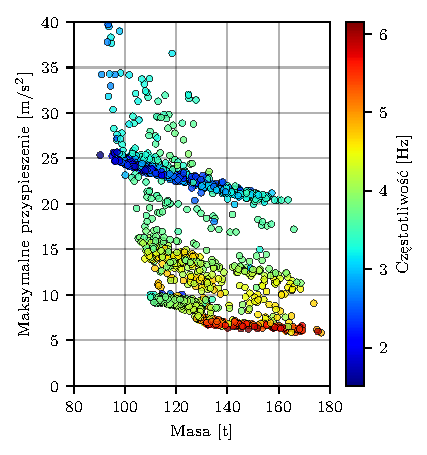
\includegraphics{proste_300_decisive_freq.pdf}}%
	\subfloat[label 2]{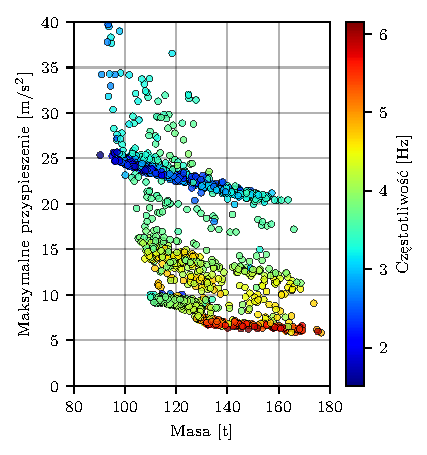
\includegraphics{proste_300_decisive_freq.pdf}}%
	\captionsetup{justification=centering}
	\caption{Częstotliwość drgań własnych związana z decydującą prędkością krytyczną. Wieszaki proste, prędkość maksymalna 300km/h}
\end{figure}
Treść dotyczącza tykresu zbiorczego 
\begin{figure}[h]
	\centering
	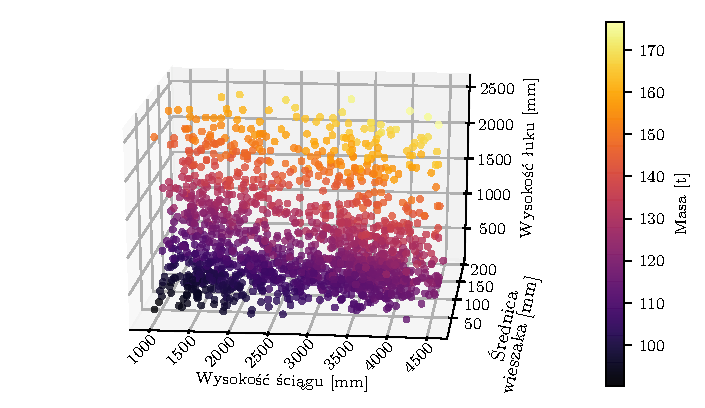
\includegraphics[width=\textwidth]{proste_300_3d_weig.pdf}
	\captionsetup{justification=centering}
	\caption{Częstotliwość drgań własnych związana z decydującą prędkością krytyczną. Wieszaki proste, prędkość maksymalna 300km/h}
\end{figure}
\begin{figure}[h]
	\centering
	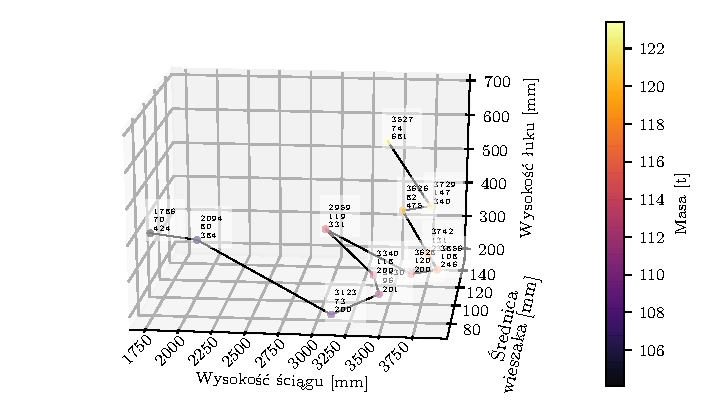
\includegraphics[width=\textwidth]{proste_300_0_3_3d_arch_weig.pdf}
	\captionsetup{justification=centering}
	\caption{Częstotliwość drgań własnych związana z decydującą prędkością krytyczną. Wieszaki proste, prędkość maksymalna 300km/h}
\end{figure}
\begin{figure}[h]
	\centering
	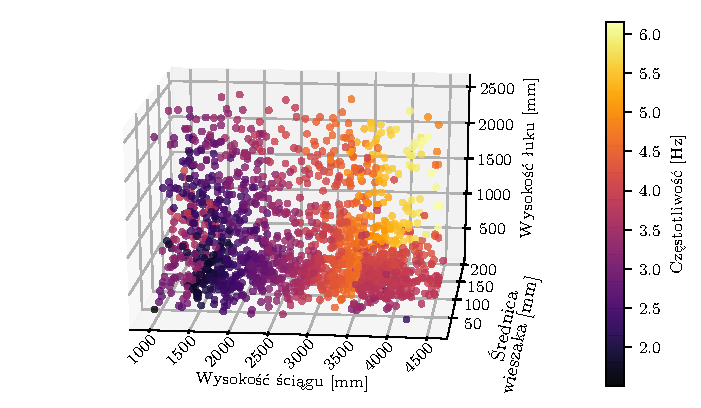
\includegraphics[width=\textwidth]{proste_300_3d_freq.pdf}
	\captionsetup{justification=centering}
	\caption{Częstotliwość drgań własnych związana z decydującą prędkością krytyczną. Wieszaki proste, prędkość maksymalna 300km/h}
\end{figure}
\begin{figure}[h]
	\centering
	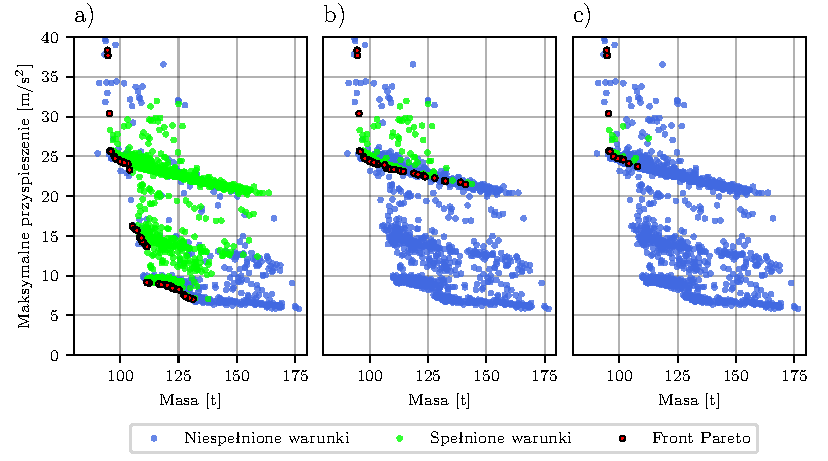
\includegraphics[width=\textwidth]{proste_300_all.pdf}
	\captionsetup{justification=centering}
	\caption{Częstotliwość drgań własnych związana z decydującą prędkością krytyczną. Wieszaki proste, prędkość maksymalna 300km/h}
\end{figure}









	\section{Typy.\\Cechy.\\Problemy związane z dynamiką.}
	\section{\textbf{Wydzielić rozdział?} Modele obiektów w celach analiz dynamicznych\\Kalibracja/Walidacja/Weryfikacja.}
\chapter{Dynamiczne obciążenie kolejowe}
	\section{Realne obciążenia - tabor.\\Modele obciążenia.\\Przepisy normowe i wytyczne.}
	
	
	
	
\chapter{Identyfikacja modalna}

Drgania towarzyszą ludzkości od zawsze. Jakkolwiek trywialnie nie brzmiałoby to zdanie, wibracje występują w naszym otoczeniu przejawiając się często w sposób niepożądany: wywołują dyskomfort użytkowania, są odbierane jako hałas, powodują zjawiska zmęczeniowe czy w skrajnej sytuacji wywołują uszkodzenia i zniszczenia \parencite{Maia1997}. Wciąż postępujący rozwój nauki połączony z komputeryzacją i informatyzacją sprawiają, że używane materiały są coraz wytrzymalsze. Jednocześnie rośnie zapotrzebowanie na coraz większe, spektakularne konstrukcje. Te dwa czynniki połączone ze sobą sprawiają, że zachowanie dynamiczne struktury często decyduje o właściwościach użytkowych i wytrzymałościowych konstrukcji. W odpowiedzi na zapotrzebowanie, w sposób naturalny rozwinęła się dziedzina nauki zajmująca się opisem i modelowaniem zjawisk dynamicznych. Podstawowym narzędziem służącym identyfikacji parametrów modalnych i zachowania dynamicznego jest analiza modalna \teng{modal analysis}. Często Analiza modalna bywa określana jako identyfikacja modalna \teng{modal identification}. \parencite{Zhang2004} w pracy definiuje identyfikacje modalną jako gałąź szerszego pojęcia identyfikacji systemów, a jej celem jest budowa modelu matematycznego systemu dynamicznego poprzez pomiar i analizę zestawu danych wejściowych i wyjściowych. Z kolei \cite{Chmielewski1998} zwięźle precyzuje pojęcie modelu matematycznego dla zagadnień dynamiki budowli jako "równanie lub zbiór równań, które opisują ruch modelu obliczeniowego". \cite{Ewins2000} podaje trzy główne cele przeprowadzania analizy modalnej:
\begin{itemize}
	\item ocena źródła drgań i ich przebiegu,
	\item weryfikacja modeli teoretycznych i przewidywanie zjawisk dynamicznych,
	\item identyfikacja charakterystyk materiałowych ciała poddanego wymuszeniu dynamicznemu (np. tłumienie, tarcie, wytrzymałość zmęczeniowa). 
\end{itemize}
Każdy z powyższych celów może być jedynie środkiem do osiągnięcia zupełnie innego celu. W rzeczywistości tak właśnie jest najczęściej o czym świadczy mnogość aplikacji analizy modalnej w bardzo różnych zagadnieniach dotyczących konstrukcji.

W poniższej pracy tak jak w zdecydowanej większości innych opracowaniach, modele matematyczne będą oparte na trzech głównych zasadach \parencite{Maia1997}:
\begin{itemize}
	\item system jest liniowy,
	\item obowiązuje zasada wzajemności Maxwell'a,
	\item system jest niezależny od czasu.
\end{itemize}


\section{Klasyfikacja metod analizy modalnej}

Identyfikacja modalna jest zbiorem technik, które są rozwijane dynamicznie od lat 60' XX w. Gwałtowny przyrost zainteresowania tym tematem wywołał głównie rozwój technik cyfrowych \parencite{Ewins2000}. Do tej pory powstało wiele różnych technik, których krótką klasyfikację z podziałem na główne kryteria podano w tym podrozdziale.

Matematyczne modele modalne mogą charakteryzować się różnym stopniem skomplikowania. Parametrami, które mogą opisywać model są postaci drgań własnych oraz powiązane z nimi częstotliwości i tłumienia modalne, a także masa i sztywność modalna. Z kolei metody analizy modalnej również różnią się pod względem informacji, którą mogą dostarczyć. Z tego względu wybór odpowiedniej metody powinien być świadomy i poparty przeglądem wielu technik, z których wybrana zostanie ta optymalna. Aspektami mogącymi wpłynąć na wybór metody są m.in.: czas potrzebny do implementacji (pierwszego użycia), informacje możliwe do uzyskania z modelu, możliwy wpływ założeń i uproszczeń, liczba parametrów potrzebnych do stworzenia modelu czy też stabilność rozwiązania. Przedstawiony podział opiera się na klasycznych kryteriach stosowanych przy klasyfikacji metod analizy modalnej. Istnieje wiele pozycji literaturowych, w których zainteresowany znajdzie dokładny opis wielu metod ze wskazówkami do ich użycia \parencite{Ewins2000,Maia1997,Zhang2004,Brincker2015,Rainieri2014}. 

Najogólniej analizę modalną można podzielić na dwie główne gałęzie zależne od typu stosowanej procedury, jej danych wejściowych i rezultatów: teoretyczną i eksperymentalną \parencite{Lengvarsky2013}. W niniejszej pracy wielokrotnie używane będą oba podejścia, dlatego autor zdecydował się na krótki ich opis. Ogólny schemat procedur teoretycznej i doświadczalnej analizy modalnej pokazano na rysunku \ref{fig:theExpProc}.  

\begin{figure}[h]
	\centering
	\subfloat[Procedura teoretyczna]{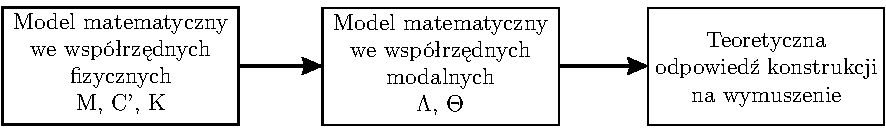
\includegraphics{/modal_analisys/schemat_theory_exper_a.pdf}
	\label{fig:theExpProcA}
	} \\
	\subfloat[Procedura doświadczalna]{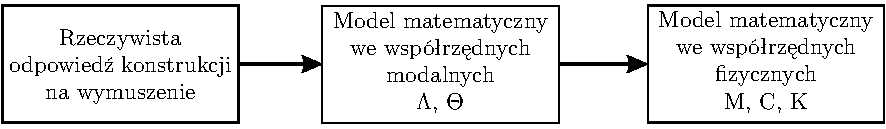
\includegraphics{/modal_analisys/schemat_theory_exper_b.pdf}
	\label{fig:theExpProcB}}
	\captionsetup{justification=centering}
	\caption{Porównanie procedur teoretycznej i doświadczalnej analizy modalnej}
	\label{fig:theExpProc}
\end{figure}

Metody teoretyczne opierają się na rozwiązaniach analitycznych lub numerycznych (rys. \ref{fig:theExpProcA}). Badanie zachowania dynamicznego rozpoczyna się od definicji struktury, najczęściej za pomocą modelu dyskretnego opisanego macierzami $\mathbf{M}, \mathbf{C}', \mathbf{K}$ oznaczającymi odpowiednio macierz mas, tłumienia i sztywności. Macierz tłumienia, w przypadku metod teoretycznych, jest to niewyznaczalna analitycznie macierz bazująca na doświadczeniach i rezultatach badań, stąd została oznaczona apostrofem $\mathbf{C'}$. Za pomocą przekształceń matematycznych (skrótowo opisanych w dalszej części tekstu) tworzony jest model matematyczny we współrzędnych modalnych. Uzyskiwane są charakterystyki modalne układu $\mathbf{\Lambda} \,\mathrm{i}\, \mathbf{\Psi}$ odpowiednio częstości drgań własnych, postaci drgań własnych i dodatkowo parametry opisujące przyjęty model tłumienia. Po uzyskaniu modelu matematycznego opisanego współrzędnymi modalnymi możliwe jest wyznaczenie odpowiedzi konstrukcji w czasie przy jej znanym wymuszeniu. Powyższy opis przedstawia pełną procedurę teoretyczną zakończoną wyznaczeniem odpowiedzi układu. Jednakże, jak wspomniano wcześniej, analiza modalna oraz jej metody są zróżnicowane z punktu widzenia skomplikowania. Zazwyczaj wybór metody zależy od zapotrzebowania na rezultaty. Zwłaszcza w przypadkach obliczeń inżynierskich często poprzestaje się na wyznaczeniu charakterystyk modalnych, które są następnie oceniane z punktu widzenia zagrożenia nadmiernymi efektami dynamicznymi.
Metody analityczne znajdują realne zastosowanie w przypadku obiektów, których opis ciągły nie jest złożony, a dyskretny ograniczony jedynie do niewielkiej liczby stopni swobody. Rzeczywiste konstrukcje są układami o nieskończonej liczbie stopni swobody. Niemniej, sprowadzenie ich do skończonej (choć zazwyczaj bardzo dużej) liczby stopni swobody pozwala otrzymać zadowalająco poprawne rezultaty. W przypadku dużej liczby stopni swobody najszerzej stosowane są metody przybliżone opierające się obliczeniach numerycznych, takie jak: metoda różnic skończonych (MRS) czy metoda elementów skończonych (MES). Teoretyczna analiza modalna ma wiele zalet. Pozwala uzyskać rezultaty relatywnie szybko i tanio. Wynika to z powszechności narzędzi do modelowania i obliczania konstrukcji. W obrębie modelowania realnych struktur współczesne oprogramowanie pozwala budować modele numeryczne praktycznie bez ograniczeń. Stosowane preprocesory graficzne pozwalają użytkownikowi na odwzorowanie nawet skomplikowanych kształtów geometrycznych. Rosnąca moc obliczeniowa komputerów przestaje być ograniczeniem, zwłaszcza przy obliczeniach statycznych modeli o znaczącej liczbie stopni swobody. Niepodważalną zaletą jest również dowolność sposobów obciążania i modyfikacji modelu numerycznego. Pomimo wielu niewątpliwych zalet, teoretyczna analiza modalna posiada ograniczenia, z których należy zdawać sobie sprawę. Przede wszystkim jakość rezultatów zależy wprost od jakości wprowadzonych przez użytkownika danych. (Potrzebne przykłady). W przypadku zagadnień dynamicznych kolejnym bardzo ważnym ograniczeniem jest brak analitycznej możliwości określenia tłumienia konstrukcji. Taką możliwość daje jedynie badanie doświadczalne na rzeczywistej konstrukcji. Metody analityczne i numeryczne są obszernie opisane w wielu publikacjach \parencite{Chmielewski1998,Chopra2012a,Rucka2014}. W dalszej części rozdziału zaprezentowano absolutne podstawy i założenia analitycznej analizy dynamicznej.


%\cite{Brincker2015} wskazuje na następujące źródła błędów i szacowane poziomy niepewności rezultatów analizy w zależności od rodzaju popełnionego błędów w definicji modelu MES (tab):

Doświadczalna analiza w odróżnieniu od wersji teoretycznej angażuje do identyfikacji warsztat badawczy. \cite{Ewins2000} definiuje ją jako zespół procesów związanych z badaniem elementów konstrukcji w celu uzyskania matematycznego opisu ich zachowania dynamicznego. Jest to definicja zbliżona do ogólniejszej podanej przez \cite{Zhang2004}, ale stawia szczególnie mocny akcent na aspekt badawczy. Jak przedstawiono na rysunku (rys. \ref{fig:theExpProcB}) ten typ analizy ma niejako odwrotny kierunek niż teoretyczna analiza modalna. W tym przypadku odpowiedź konstrukcji jest mierzona i na jej podstawie wyznaczane są wielkości opisujące model matematyczny: $\mathbf{\Lambda}$ i $\mathbf{\Psi}$. Następnie na dopiero ich podstawie możliwe jest przekształcenie na model matematyczny wyrażony we współrzędnych fizycznych: $\mathbf{M}, \mathbf{C}', \mathbf{K}$. 
Doświadczalna analiza modalna dzieli się na dwie główne odnogi związane z zakresem rejestrowanych danych w trakcie wykonywania eksperymentu. Pierwsza z nich to Eksperymentalna Analiza Modalna (EMA) \teng{Experimental Modal Analysis} wymaga pomiaru sił wymuszających oraz odpowiedzi konstrukcji na to wymuszenie. Druga to Operacyjna Analiza Modalna (OMA) \teng{Operational Modal Analysis}, która estymuje parametry modalne wyłącznie na podstawie pomierzonych efektów nieznanego wymuszenia. Wymuszenie to jednak nie może być dowolne, a ograniczenia przedstawione zostaną w dalszej części pracy. 

Kwestia pomiaru sił wymuszających wpływa na podstawowe różnice pomiędzy dwoma rodzinami metod: EMA i OMA. EMA najczęściej prowadzona jest w kontrolowanych warunkach i przez to pozwala dostarczyć bardziej szczegółowych i dokładniejszych informacji na temat zachowania dynamicznego konstrukcji. Jednakże w przypadku rzeczywistych konstrukcji inżynierskich (np. mosty) trudno jest stworzyć takie kontrolowane warunki. Obiekt musi zostać na czas pomiarów wyłączony z eksploatacji. Okazuje się to często niemożliwe z przyczyn proceduralnych, a na pewno kosztowne. Drugim zasadniczym ryzykiem jest potrzeba stworzenia takiego systemu wymuszenia, które wywoła mierzalną odpowiedź konstrukcji. W przypadku dużych konstrukcji inżynierskich może okazać się to trudne do zrealizowania ponieważ oddziaływania środowiskowe mogą wywoływać efekty oddziaływań porównywalne z kontrolowanym wymuszeniem. OMA praktycznie pozbywa się negatywnych skutków potrzeby kontroli wymuszenia. Badania prowadzone mogą być przy normalnej eksploatacji, a losowe oddziaływania środowiskowe zazwyczaj polepszają jakość wyników. Oczywiście odbywa się to kosztem dokładności rezultatów. Teoretyczne założenia metody są spełnione tylko w sposób przybliżony. Z tego względu serie pomiarowe zwykle muszą trwać znacznie dłużej, a interpretacja wyników wymaga większego doświadczenia.

\textbf{Połączenie obu typów analiz}

\section{Teoretyczna analiza modalna}
\label{section: eigen}
Metody teoretycznej analizy modalnej są obszernie opisane w literaturze przedmiotu (cytowania). Ze względu na złożoność rzeczywistych konstrukcji, w praktyce mają one zastosowanie głównie w formie rozwiązań numerycznych.  Według przedstawionej na rysunku \ref{fig:theExpProcA} procedury metody teoretycznej analizy modalnej służą głównie dwóm celom: identyfikacji charakterystyk modalnych (częstotliwości i postaci drgań własnych) i wyznaczaniu odpowiedzi układu. Dla zrozumienia zagadnienia, metody analityczne najczęściej przedstawione są dla najprostszego przypadku układu z jednym stopniem swobody. Układ ten z reguły łatwo daje się uogólnić do układu o wielu stopniach swobody. Macierzowe równanie drgań wymuszonych dla tłumionego układu o skończonej liczbie stopni swobody przedstawiono we wzorze \ref{eq: mot_und}. 
\begin{equation} \label{eq: mot_und}
\vect{M} \vect{\ddot{x}}(t) +\vect{C} \vect{\dot{x}}(t)+ \vect{Kx}(t) = \vect{F}(t)
\end{equation}
gdzie $\vect{M},\vect{C},\vect{K}$ to odpowiednio macierze mass, tłumienia i sztywności, $\vect{x}$ to wektor współrzędnych uogólnionych (przemieszczeń lub obrotów punktu), $\vect{F}(t)$ to wektor uogólnionych sił wymuszających. Wzór \ref{eq: mot_dam} odpowiadający formule \ref{eq: mot_und} pozbawionej składnika reprezentującego opory ruchu opisuje ruch nietłumiony układu. 
\begin{equation} \label{eq: mot_dam}
\vect{M} \vect{\ddot{x}}(t) +\vect{Kx}(t) = \vect{F}(t)
\end{equation}

Drgania swobodne są procesem fizycznym spowodowanym zaburzeniem stanu równowagi, przez zaistnienie warunków początkowych. Macierzowe równanie ruchu drgań swobodnych, tłumionych opisane jest wzorem \ref{eq: mot_dam_free}, a nietłumionych wzorem \ref{eq: mot_und_free}. Od równań ruchu drgań wymuszonych, równania te różnią się brakiem składnika sił wymuszających.
\begin{equation} \label{eq: mot_dam_free}
\vect{M} \vect{\ddot{x}}(t) +\vect{C} \vect{\dot{x}}(t)+ \vect{Kx}(t) = \vect{0}
\end{equation}

\begin{equation} \label{eq: mot_und_free}
\vect{M} \vect{\ddot{x}}(t) +\vect{Kx}(t) = \vect{0}
\end{equation}


Okazuje się, że parametry modalne systemu są ściśle powiązane z rozwiązaniem algebraicznego problemu własnego równań drgań własnych. 

\subsection{Zagadnienie własne}
Identyfikacja modalna modelu matematycznego polegająca na wyznaczeniu częstotliwości i postaci drgań własnych najczęściej sprowadza się do rozwiązania zagadnienia własnego. Bardzo pozytywnym aspektem tej zależności jest to, że istnieje wiele prostych w aplikacji, wydajnych i dokładnych algorytmów pozwalających rozwiązać numerycznie zagadnienie własne \parencite{Golub2013}. Dzięki temu, właśnie ta metoda identyfikacji modalnej cieszy się największą popularnością wśród producentów oprogramowania do obliczania konstrukcji. Użytkownicy oprogramowania mogą bez większego wysiłku dokonać identyfikacji parametrów modalnych nawet złożonych modeli matematycznych. 
\subsubsection{Układ nietłumiony}
Z reguły przyjmuje się, że rozwiązanie zagadnienia własnego wykorzystuje równanie drgań swobodnych nietłumionych (\ref{eq: mot_und_free}). Należy zaznaczyć, że drgania własne nie opisują procesu fizycznego, a są jedynie matematyczną idealizacją drgań układu. W przypadku nietłumionym, dla każdego z modów, układ oscyluje wokół położenia równowagi z częstotliwością drgań własnych, a wszystkie stopnie swobody drgają w tej samej fazie. Oznacza to, że każdy z punktów osiąga swoje ekstremalne położenie w tej samej chwili. Podobnie wszystkie punkty znajdują się w położeniu równowagi w tym samym czasie. Poniżej przedstawiono rozwiązanie dla nietłumionego układu $N$ dynamicznych stopni swobody.

Założono rozwiązanie \ref{eq: mot_und_free} w postaci $\vect{x}(t)=\vect{\psi}e^{j\omega t}$ gdzie $\omega$ to częstość drgań własnych, $j=\sqrt{-1}$, a $\psi$ to niezerowy wektor postaci drgań własnych. Po podstawieniu rozwiązania i jego drugiej pochodnej ($\vect{\ddot{x}}(t)=-\vect{\psi} \omega^2 e^{j\omega t}$) do równia \ref{eq: mot_und_free} otrzymamy równanie \ref{eq: char_equation1}.

\begin{equation} \label{eq: char_equation1}
-\vect{M}\vect{\psi}\omega^2 e^{j\omega t} +\vect{K\psi}e^{j\omega t} = \vect{0}
\end{equation}
Dzieląc strony równania przez niezerową wartość $e^{j\omega t}$ otrzymujemy układ liniowych równań algebraicznych:
\begin{equation} \label{eq: char_equation2}
-\vect{M}\omega^2 \vect{\psi} +\vect{K\psi} = \vect{0}
\end{equation}
w którym dwie niewiadome do ustalenia to: $\psi$ - niezerowy wektor postaci drgań własnych oraz $\omega$ - częstość drgań własnych. Równanie to można zapisać w formie \ref{eq: char_equation3} z indeksami określającymi poszczególne mody drgań własnych. Liczba par odpowiadających sobie częstości $\omega_i$ i postaci drgań własnych $\psi_i$ jest równa liczbie $N$ stopni swobody. 
\begin{equation} \label{eq: char_equation3}
\omega^2_i \vect{M}\psi_i = \vect{K}\psi_i\qquad i=1,2,...,N
\end{equation}
Z kolei równanie \ref{eq: char_equation4} to reprezentacja uogólnionego problemu własnego, w którym $\lambda_i$ to wartość własna, a $u_i$ to wektor własny. Z porównania wzorów \ref{eq: char_equation3} i \ref{eq: char_equation4} wyraźnie widać powiązanie $\lambda_i=\omega^2_i$. Wynika z tego, że rozwiązanie numeryczne uogólnionego problemu własnego pozwala wprost uzyskać częstości $(\lambda_i=\omega^2_i)$ i postaci drgań własnych $(\psi_i)$. 
\begin{equation} \label{eq: char_equation4}
\lambda_i \vect{A}u_i = \vect{B}u_i
\end{equation}
Układ równań (\ref{eq: char_equation3}) ma nietrywialne rozwiązania tylko jeśli
\begin{equation} \label{eq: char_equation_det}
\det[\vect{K}-\omega^2_i \vect{M}] = \vect{0}
\end{equation}
Formuła \ref{eq: char_equation_det} jest znana jako równanie charakterystyczne zagadnienia własnego. Jeśli rozwinąć wyznacznik, otrzymamy wielomian stopnia $N$ względem $\omega^2_i$. Pierwiastkami równania \ref{eq: char_equation_det} są częstości drgań własnych $\omega_i$. Znając częstości własne $\omega_i$ z równania \ref{eq: char_equation3} można obliczyć odpowiadające wektory własne $\psi_i$ z dokładnością do stałego czynnika. Taki wynik bywa nieprzystępny w ocenie więc wektory poddawane mogą być normalizacji. Do najczęściej stosowanych metod normalizacji należy taka modyfikacja wektora tak aby maksymalna wartość bezwzględna spośród wszystkich elementu była równa jedności. Innym przykładem może być normalizacja wektorów tak aby wartość elementu dla danego stopnia swobody, we wszystkich wektorach była równa jedności.

Jeżeli macierze $\vect{M}$ i $\vect{K}$ ($\vect{A}$ i $\vect{B}$ wg \ref{eq: char_equation2}) są symetryczne i dodatnio określone o wartościach rzeczywistych to wartości oraz wektory własne są również rzeczywiste. W przypadku konstrukcji budowlanych macierz $\vect{K}$ jest zawsze dodatnio określona ponieważ warunki brzegowe zapewniają brak ruchu ciała jako bryły sztywnej. Nie jest to oczywiste dla innych niż budowlane struktur, takich jak np. samolot w locie \parencite{Chopra2012a}.


Postaci drgań własnych (wektory własne) odpowiadające różnym częstościom własnym spełniają warunki ortogonalności. W przypadku gdy $\omega_i \neq \omega_j$ prawdziwe są zależności \ref{eq: eigenvect_orto}. Ortogonalność wektorów własnych może być wykorzystana do weryfikacji obliczonych wektorów. 
\begin{equation} \label{eq: eigenvect_orto}
\vect{\psi}_i^{T}\vect{K\psi}_j = 0 \qquad \vect{\psi}_i^{T}\vect{M\psi}_j = 0
\end{equation}

Obliczone z równania \ref{eq: char_equation_det} wartości oraz wektory własne możemy przedstawić w postaci dwóch specjalnych macierzy. $N$ obliczonych wartości własnych zestawionych w macierz diagnonalną tworzy tak zwaną macierz widmową (\ref{eq: mat_spect}). Z kolei $N$ wektorów własnych zestawionych kolumnowo nazywamy macierzą modalną (\ref{eq: mat_modal}).

\begin{equation}  \label{eq: mat_spect}
\vect{\Omega}^2 =  
\begin{bmatrix} 
	\omega_{1}^2 & 0 			& \dots  & 0      \\ 
	0 		     & \omega_{2}^2 & \dots  & 0      \\
	\vdots       & \vdots       & \ddots & \vdots \\
	0 			 & 0 		    & \dots  & \omega_{N}^2 


\end{bmatrix}
\end{equation}

\begin{equation} \label{eq: mat_modal}
	\vect{\Psi} = [\psi_{i,j}]= 
	\begin{bmatrix} 
		\psi_{11} & \psi_{12} & \dots & \psi_{1N} \\ 
		\psi_{12} & \psi_{22} & \dots & \psi_{2N} \\
		\vdots    & \vdots    & \ddots & \vdots \\
		\psi_{N1} & \psi_{N2} & \dots & \psi_{NN} 
	
	
	\end{bmatrix}
	\qquad
	1\leq i,j \leq N.
\end{equation}

Dla układu o $N$ stopniach swobody możemy wyznaczyć $N$ par częstotliwości i postaci drgań własnych. Jednak w rzeczywistości rozwiązanie ogranicza się do wyznaczenia jedynie ograniczonej do kilkunastu (maksymalnie kilkuset) pierwszych par. Określenie "pierwszych" właściwe jest w przypadku kiedy wyznaczone częstości uporządkujemy w szeregu rosnącym
\begin{equation} \label{eq: eigenvalues_list}
0 \leq \omega_1  \leq \omega_2 \dots  \omega_{N-1} \leq  \omega_N
\end{equation}

W większości przypadków zagadnienie własne jest rozwiązywane numerycznie za pomocą maszyn cyfrowych. Metody numeryczne wykorzystują iteracyjne algorytmy do rozwiązania zagadnienia własnego. \cite{Chopra2012a} definiuje trzy główne kategorie algorytmów: 
\begin{itemize}
	\item Metody iteracji wektora wykorzystujące właściwości równania (\ref{eq: char_equation3}),
	\item Metody transformacyjne korzystające z ortogonalności wektorów własnych,
	\item Metody iteracyjne wykorzystujące równanie charakterystyczne (\ref{eq: char_equation_det}).
\end{itemize}
Dla dużych systemów korzystne okazuje się łączenie algorytmów z tej samej bądź różnych kategorii co podnosi wydajność metody rozwiązania. W oprogramowaniu komercyjnym stosowane są złożone algorytmy takie jak metoda iteracji podprzestrzeni, metoda Lanczosa czy metoda gradientów Ritza. Wybór metody zależy również od wybranego solvera (silnika programu rozwiązującego równania). Algorytmy te różnią się pod względem wydajności, maksymalnej dokładności rozwiązania czy zbieżności. Ich wydajność może zależeć od liczby zadanych do wyznaczenia wartości własnych czy wielkości zadania. Więcej szczegółów odnośnie stosowanych metod rozwiązania zagadnienia własnego można odnaleźć w literaturze \parencite{Bathe2006,Wilson1983,Wilson1997,Fialko2000,Papadrakakis1993,Hughes1987,Chopra2012a}. W przypadku dobrej jakości oprogramowania komercyjnego informacje na temat używanych algorytmów powinny dostępne w pomocy do programu.

\subsubsection{Układ tłumiony}
Drgania swobodne tłumione układu określone są równaniem (\ref{eq: mot_dam_free}), które przytoczono ponownie poniżej:
\begin{equation} \label{eq: mot_dam_free2}
\vect{M} \vect{\ddot{x}}(t) +\vect{C} \vect{\dot{x}}(t)+ \vect{Kx}(t) = \vect{0}
\end{equation}
Rozwiązanie tego równania jest uzależnione od postaci tłumienia: klasycznego lub nieklasycznego. Tłumienie klasyczne zwane również proporcjonalnym \teng{classical damping, proportional damping} występuje w przypadku kiedy spełnione jest równanie (\ref{eq: class_damp}). 
\begin{equation} \label{eq: class_damp}
\vect{CM}^{-1}\vect{K} = \vect{KM}^{-1}\vect{C}
\end{equation}
Kiedy macierz $\vect{C}$ jest diagonalna to warunek (\ref{eq: class_damp}) jest spełniony. W takim przypadku wszystkie częstości drgań własnych są rzeczywiste i identyczne do tych wyznaczonych dla układu nietłumionego. W przypadku przeciwnym mamy do czynienia z tłumieniem nieklasycznym bądź nieproporcjonalnym \teng{nonclassical damping, nonproportional damping}. Dla tej sytuacji macierz $\vect{C}$ nie jest diagonalna, a wartości własne są zespolone. Szczegółowe informacje oraz metody rozwiązania przypadków dynamiki konstrukcji nieklasycznie tłumionych podano w \parencite{Caughey1961,Chopra2012a}. \cite{Inman1995} na przykładzie pokazali, że obliczanie struktur charakteryzujących się tłumieniem nieklasycznym za pomocą zagadnienia własnego bez uwzględnienia macierzy tłumienia możne prowadzić do błędnych rezultatów. Tak wyznaczone częstotliwości drgań będą różnić się od rzeczywistych, co może pociągnąć za sobą błędne wnioski odnośnie zakresu częstotliwości grożących rezonansem.
\subsection{Transformacja do współrzędnych normalnych} \label{section: transform_normal}
Rozważmy ponownie równanie ruchu układu MDOF (\ref{eq: mot_dam_free2}). Wiemy, że każdy wektor o długości $N$ może być przedstawiony jako kombinacja liniowa $N$ liniowo niezależnych wektorów. Przedstawmy zatem wektor przemieszczeń $\vect{x}$ jako kombinację wektorów własnych $\vect{\psi}$.
\begin{equation} \label{eq: normal_coord_komb}
	\vect{x} = \sum_{r=1}^{N} \vect{\psi}_r q_r=\vect{\Psi q}
\end{equation} 
gdzie współczynniki $q_r$ nazywane są współrzędnymi normalnymi \teng{modal coordinates, normal coordinates} i $\vect{q}=<q_1\,\,q_2\,\, \dots\,\, q_N>^T$. Załóżmy, że zagadnienie własne zostało rozstrzygnięte i wyznaczyliśmy macierz modalną $\vect{\Psi}$ (\ref{eq: mat_modal}). Aby uzyskać wartości współczynników $q_n$ dla danego $\vect{x}$, przemnóżmy obie strony równania \ref{eq: normal_coord_komb} przez $\vect{\psi}_n^T\vect{M}$:
\begin{equation} \label{eq: normal_coord_komb2}
	\vect{\psi}_n^T\vect{M}\vect{x} = \sum_{r=1}^{N} (\vect{\psi}_n^T\vect{M}\vect{\psi}_r) q_r
\end{equation} 

Ortogonalność wektorów własnych (\ref{eq: eigenvect_orto}) sprawia, że wszystkie składniki powyższej sumy są równe 0 poza tymi, w których $r=n$. Pomińmy więc znak sumy i zapiszmy 
\begin{equation} \label{eq: normal_coord_kom3}
	\vect{\psi}_n^T\vect{M}\vect{x} = (\vect{\psi}_n^T\vect{M}\vect{\psi}_n) q_n
\end{equation} 

\begin{equation} \label{eq: normal_coord_kom4}
	q_n = \frac{\vect{\psi}_n^T\vect{M}\vect{x}}{\vect{\psi}_n^T\vect{M}\vect{\psi}_n} 
\end{equation} 
Transformacja do współrzędnych normalnych jest istotnym elementem przewidywania odpowiedzi wymuszonych, liniowych układów MDOF z tłumieniem proporcjonalnym (p. \ref{section: mdof_response}).

%Należy wspomnieć, że uogólniony problem własny nie jest jedyną metodą rozwiązania macierzowego równania ruchu. Przy spełnieniu powyższych warunków możliwe jest również przekształcenie uogólnionego problemu własnego w odpowiedni standardowy (prosty) problem własny:
%\begin{equation} \label{eq: eige_stan_1}
%\vect{A}u_i = \lambda_i u_i
%\end{equation}
%Aby doprowadzić równanie \ref{eq: char_equation3} do postaci standardowego problemu własnego wymagane jest wyznaczenie macierzy odwrotnej $\vect{M}^{-1}$. W przypadku kiedy jest to możliwe (na przykład przy pomocy dekompozycji Choleskiego) należy pomnożyć lewostronnie strony równania przez $\vect{M}^{-1}$ co pozwala uzyskać postać (\ref{eq: eige_stan_2}). Ponownie widoczne jest podobieństwo pomiędzy równaniami i powiązanie $(\lambda_i=\omega^2_i)$. Sprowadzenie do standardowego problemu własnego bywa korzystne z punktu widzenia rozwiązania numerycznego. 
%\begin{equation} \label{eq: eige_stan_2}
%\vect{M}^{-1}\vect{K}\psi_i=\omega^2_i\psi_i
%\end{equation}

\subsection{Odpowiedź systemów dynamicznych o jednym stopniu swobody} \label{section: sdof_response}

Przegląd metod pozwalających wyznaczyć odpowiedź konstrukcji poddanej wymuszeniu wypada zacząć klasycznie od układu z jednym stopniem swobody. W przypadku liniowego układu SDOF obciążonego siłą zewnętrzną, równanie ruchu jest liniowym równaniem różniczkowym drugiego rzędu (\ref{eq: eq_mot_sdof}). Znając warunki początkowe $x(0)$ i $\dot{x}(0)$ możemy traktować zadanie jako w pełni sformułowane. Dla konstrukcji wstępnie nieobciążonej dynamicznie przemieszczenie i prędkość początkowe można przyjąć jako równe zeru.
\begin{equation} \label{eq: eq_mot_sdof}
	m\ddot{x}+c\dot{x}+k{x}=f(t)
\end{equation}
Dla tak sformułowanego problemu istnieją cztery podstawowe metody wyznaczenia odpowiedzi dynamicznej:
\begin{itemize}
	\item klasyczne rozwiązanie równań różniczkowych,
	\item wykorzystanie całki Duhamela,
	\item rozwiązanie w dziedzinie częstotliwości,
	\item wykorzystanie metod numerycznych.
\end{itemize}
Dla porządku powyższe metody zostaną w dalszej części krótko opisane. Dokładny opis metod jest przedstawiony w wielu podstawowych pozycjach literaturowych dotyczących dynamiki budowli \parencite{Clough1975,Chmielewski1998,Chopra2012a}.

\subsubsection{Metoda klasyczna}

Rozwiązanie liniowego równania różniczkowego o stałych współczynnikach jakim jest równanie ruchu składa się z rozwiązania całki ogólnej i szczególnej, a następnie zsumowaniu ich. Równanie ruchu jest rzędu drugiego stąd do wyznaczenia pozostają dwie zmienne całkowania. Z kolei do ich wyznaczenia wykorzystane są warunki początkowe. $\bm{OGRANICZENIA}$

\subsubsection{Całka Duhamela}

Metoda rozwiązania równania ruchu układu SDOF za pomocą całki Duhamela polega na przekształceniu funkcji obciążenia $f(t)$ na sekwencję nieskończenie krótkich impulsów. Przykładając impulsowe, jednostkowe wymuszenie (delta Diraca) do układu (\ref{eq: eq_mot_sdof}), dla odpowiednich warunków początkowych otrzymuje się rozwiązanie w postaci odpowiedzi impulsowej, inaczej zwanej impulsową funkcją przejścia \teng{unit response function}. Aby uzyskać odpowiedź układu w czasie $t$ sumuje się wszystkie odpowiedzi impulsowe do chwili czasowej $t$. W przypadku całkowalnej funkcji wymuszenia, całka Duhamela może być alternatywą do rozwiązania metodą klasyczną. Dla eksperymentalnych funkcji wymuszenia, całkę Duhamela można wyznaczyć metodami numerycznymi. W tym przypadku odpowiedź będzie wyznaczona w dyskretnych chwilach czasowych. Należy jednak wspomnieć, w przypadku angażowania metod numerycznych całka Duhamela nie jest najwydajniejszym rozwiązaniem. Dodatkowo, ze względu na wykorzystywaną superpozycję, rozwiązanie to jest ograniczone wyłącznie do układów liniowych.

\subsubsection{Metoda przejścia do dziedziny częstotliwości}

Metoda przejścia do dziedziny częstotliwości \teng{frequency-domain method} wykorzystuje właściwości przekształceń Laplace'a lub Fourier'a. Dla układu SDOF (\ref{eq: eq_mot_sdof}) wykonuje się wybrane przekształcenie funkcji wymuszenia $f(t)$ uzyskując $F(\omega)$. $F(\omega)$ można określić jako amplitudy wszystkich składników harmonicznych, które składają się na wymuszenie $f(t)$ Przekształcenie $X(\omega)$ rozwiązania równania różniczkowego $x(t)$ można z kolei opisać następująco
\begin{equation}
	X(\omega)=H(\omega)F(\omega)
\end{equation}
gdzie $H(\omega)$ to odpowiedź zespolona w dziedzinie częstotliwości nazywana też funkcją przenoszenia lub transmitancją \teng{complex frequency-response function (FRF)}. Funkcja przenoszenia $H(\omega)$ opisuje odpowiedź układu w dziedzinie częstotliwości przy wymuszeniu harmonicznym. Ostatnim krokiem metody jest wyznaczenie rozwiązania $x(t)$ poddając $X(\omega)$ odwrotnemu przekształceniu (Fourier'a bądź Laplace'a). Tak uzyskany rezultat $x(t)$ można traktować jako określenie odpowiedzi harmonicznych układu na każdy z składników wymuszenia. Te cząstkoweg odpowiedzi te są następnie sumowane w celu uzyskania całkowitej odpowiedzi $x(t)$. Ponownie, metoda ta bezpośrednio może być stosowana tylko dla prostych funkcji wymuszenia $f(t)$. Jeżeli funkcja wymuszenia jest określona numerycznie, odpowiednie przekształcenia można przeprowadzić np. z użyciem algorytmu dyskretnej transformaty Fouriera w wariancie szybkiej transformaty Fourier'a \teng{Fast Fourier Transform (FFT)}.

\subsubsection{Metody numeryczne}

Zastosowanie powyższych trzech metody wyznaczania odpowiedzi dynamicznej ograniczone jest tylko do układów liniowych. Wspomniano również, że stają się niepraktyczne lub wręcz niemożliwe do zastosowania w przypadku skomplikowanych, zmiennych w czasie funkcji wymuszenia $f(t)$. W takich niekorzystnych okolicznościach z pomocą przychodzą metody numeryczne. Co więcej, okazuje się, że w przypadkach liniowych układów metody te są również konkurencyjne dla metod analitycznych. 

Stworzono wiele metod i algorytmów numerycznych służących skutecznemu rozwiązaniu równań ruchu. Powstało wiele pozycji traktujących o tym zagadnieniu (LITERATRA). Z tego względu przytoczono tylko podstawowe pojęcia i założenia dotyczące istoty rozwiązań numerycznych układów SDOF. Metody numeryczne w głównej mierze opierają się na mechanizmie kroku czasowego \teng{time-step}. Polega on na dyskretyzacji siły wymuszającej i odpowiedzi układu poprzez określenie ich wyłącznie w wybranych chwilach czasowych. Rozpatrzmy równanie ruchu SDOF:
\begin{equation}
	m\ddot{x}+c\dot{x}+kx = f(t)
\end{equation} 
Dokonajmy dyskretyzacji i przedstawmy siłę wymuszającą $f(t)$ określoną dla $t\in<0,t_k>$ jako zestaw dyskretnych wartości w chwilach czasowych $t_i$:
\begin{equation}
	f_i=f(t_i) \qquad i = 0,1,2\dots N-1,N
\end{equation}
gdzie $t_N\leq t_k$. Krokiem czasowym nazywamy różnice pomiędzy kolejnymi zdyskretyzowanymi chwilami czasowymi:
\begin{equation}
	\Delta t_i = t_{i+1}-t_i
\end{equation}
Jest on zazwyczaj przyjmowany jako stały, ale nie jest to konieczne. Tak jak wymuszenie, odpowiedź również podlega dyskretyzacji w chwilach $t_i$, a więc równanie ruchu można zapisać w nowej formie
\begin{equation}
	m\ddot{x}_i+c\dot{x}_i+kx_i = f_i
\end{equation}
Znając warunki początkowe $x(0)$ i $\dot(x)(0)$ algorytmy wykorzystywane w metodach numerycznych potrafią wyznaczyć rozwiązania równania w kolejnych krokach $i = 1,2\dots N-1,N$. Zwykle jednak nie jest to rozwiązanie ścisłe. Metody dostarczają przybliżonych rozwiązań, dlatego też muszą spełniać następujące kryteria:
\begin{itemize}
	\item zbieżności \teng{convergence} - wraz ze zmniejszeniem kroku czasowego, rozwiązanie powinno zmierzać do rozwiązania dokładnego,
	\item stabilności \teng{stability} - rozwiązanie powinno być stabilne pomimo występowania błędów zaokrągleń,
	\item dokładności \teng{accuracy} - rozwiązanie powinno być dostatecznie bliskie rozwiązanie dokładnego.
\end{itemize}
Wśród metod numerycznych, które okazały się skuteczne w rozwiązaniach problemów możemy wyróżnić trzy główne:
\begin{itemize}
\item metoda interpolacji funkcji wymuszającej,
\item metoda różnic skończonych,
\item metoda średniego lub liniowego przyspieszenia w przedziale różnicowym, oparte na metodzie Newmark'a.
\end{itemize}
Pomimo, że powyższe metody są opisane dla układu SDOF, są praktycznie wykorzystywane do obliczania układów MDOF. Poniżej przedstawiono metody wyznaczania odpowiedzi dla układów MDOF. 


\subsection{Odpowiedź systemów dynamicznych o skończonej liczbie stopni swobody (MDOF)} \label{section: mdof_response}

Systemy o skończonej liczbie stopni swobody mogą charakteryzować się tłumieniem klasycznym (proporcjonalnym) bądź nieklasycznym (nieproporcjonalnym). Mogą być liniowe lub nieliniowe geometrycznie lub materiałowo. Czynniki te mają wpływ na wybór metody przewidywania odpowiedzi takiego układu. Macierzowe równanie ruchu dla układu o $N$ stopniach swobody możemy zapisać jako $N$ równań różniczkowych w formie (\ref{eq: mot_und}) dla wygody ponownie opisanej równaniem (\ref{eq: mot_und_num})
\begin{equation} \label{eq: mot_und_num}
	\vect{M} \vect{\ddot{x}}(t) +\vect{C} \vect{\dot{x}}(t)+ \vect{Kx}(t) = \vect{F}(t)
\end{equation}
 Modelem z tłumieniem proporcjonalnym, z wystarczającym przybliżeniem, można opisać większość badanych struktur. Odpowiedź układów ograniczonych do kilku stopni swobody może być wyznaczana przez rozwiązanie równania różniczkowego \ref{eq: mot_und_num}. W przypadku większej liczby stopni swobody zwykle wykorzystuje się metody numeryczne. Jak wiemy z rozdziału \ref{section: eigen}, dla takich układów zawsze możliwe jest wyznaczenie częstotliwości i postaci drgań własnych. Co więcej, opisujące je macierzowe równanie ruchu można przekształcić za pomocą metody transformacji własnej do postaci zależnej od współrzędnych modalnych. W takiej formie równanie to jest zbiorem równań rozwikłanych. Z tego względu można wyznaczyć odpowiedź dla każdego modu (zestawu jednej częstotliwości i postaci własnej oraz towarzyszącego tłumienia) osobno, a następnie złożyć je w celu wyznaczenia odpowiedzi całkowitej. Dodatkowo, każda odpowiedź modalna może być wyznaczona jako funkcja czasu przez analizę układu SDOF. Równania SDF mogą być oczywiście rozwiązane wszystkimi przytoczonymi wcześniej wymienionymi metodami - w tym numerycznymi.
 
 W przypadku kiedy mamy do czynienia z układem o tłumieniu nieproporcjonalnym, klasyczne parametry modalne nie mogą być wyznaczone, a równania ruchu nie mogą być rozwikłane. Takie systemy można analizować dwiema metodami: poprzez przekształcenie równań ruchu na wektory własne obliczone w zespolonym zagadnieniu własnym lub poprzez bezpośrednie całkowanie nierozwikłanych równań różniczkowych. Druga metoda wykorzystuje metody numeryczne co wynika z braku zamkniętych rozwiązań analitycznych nawet dla analitycznie opisanych funkcji obciążenia. Metody numeryczne muszą być stosowane również w przypadku kiedy układ jest nieliniowy (niezależnie czy materiałowo, czy geometrycznie). W przypadku braku założenia o liniowości wybór metody nie jest uzależniony od tego, czy tłumienie jest proporcjonalne, czy też nie jest.
 
 Zachowując porządek i kompletność wywodu poniżej przedstawiono krótki zarys dwóch podstawowych metod wyznaczania odpowiedzi układów dyskretnych o skończonej liczbie stopni swobody.
 
 \subsubsection{Metoda superpozycji modalnej}
Rozpatrzmy układ MDOF, liniowy o tłumieniu proporcjonalnym dany równaniem \ref{eq: mot_und_num}. Wiemy, że wektor przemieszczeń $\vect{x}$ może być zapisany za pomocą współrzędnych normalnych (p. \ref{section: transform_normal}) co powtórzono dla wygody poniżej:

\begin{equation} \label{eq: superposition_modal_1_przytocz}
	\vect{x}(t) = \sum_{r=1}^{N} \vect{\psi}_r q_r(t)=\vect{\Psi q}(t)
\end{equation} 

Podstawmy \ref{eq: superposition_modal_1} do równania \ref{eq: mot_und_num}
\begin{equation} \label{eq: superposition_modal_2_podstaw}
	\sum_{r=1}^{N} \vect{M} \vect{\psi}_r \ddot{q}_r(t) +\sum_{r=1}^{N} \vect{C}\vect{\psi}_r \dot{q}_r(t) + \sum_{r=1}^{N} \vect{K}\vect{\psi}_r q_r(t) = \vect{F}(t)
\end{equation} 
Następnie przemnóżmy z lewej strony każdy składnik przez $\vect{\psi}_n^T$ otrzymując:
\begin{equation} \label{eq: superposition_modal_3_przemnoz}
	\sum_{r=1}^{N} \vect{\psi}_n^T \vect{M} \vect{\psi}_r \ddot{q}_r(t) +\sum_{r=1}^{N} \vect{\psi}_n^T \vect{C}\vect{\psi}_r \dot{q}_r(t) + \sum_{r=1}^{N} \vect{\psi}_n^T \vect{K}\vect{\psi}_r q_r(t) = \vect{\psi}_n^T \vect{F}(t)
\end{equation} 
Podobnie jak w punkcie \ref{section: transform_normal}, ortogonalność wektorów własnych $\vect{\psi}$ sprawia, że wszystkie składniki sum, w których $r\neq n$, zerują się. Możemy więc zapisać zredukowane równanie w postaci
\begin{equation} \label{eq: superposition_modal_4_orto}
	 (\vect{\psi}_n^T \vect{M} \vect{\psi}_n )\ddot{q}_n(t) + (\vect{\psi}_n^T \vect{C}\vect{\psi}_n) \dot{q}_n(t) + (\vect{\psi}_n^T \vect{K}\vect{\psi}_n) q_n(t) = \vect{\psi}_n^T \vect{F}(t)
\end{equation} 
Zauważmy, że iloczyny zawarte w nawiasach są skalarami. Uprośćmy więc zapis do następującej formy:
\begin{equation} \label{eq: superposition_modal_5_uprosc}
	\mathcal{M}_n\ddot{q}_n(t) + \mathcal{C}_n\dot{q}_n(t) + \mathcal{K}_n q_n(t) = \mathcal{F}_n(t)
\end{equation} 
gdzie:
\begin{equation} \label{eq: superposition_modal_6_podstawki}
	\mathcal{M}_n= \vect{\psi}_n^T \vect{M} \vect{\psi}_n \qquad 
	\mathcal{C}_n= \vect{\psi}_n^T \vect{C} \vect{\psi}_n \qquad 
	\mathcal{K}_n= \vect{\psi}_n^T \vect{K} \vect{\psi}_n \qquad
	\mathcal{F}_n(t)= \vect{\psi}_n^T \vect{F}(t)
\end{equation} 
Okazuje się, że wszystkie powyższe przekształcenia doprowadzają do tego, że (\ref{eq: superposition_modal_5_uprosc}) jest równaniem o jednym stopniu swobody dla $n$-tej współrzędnej normalnej odpowiadającej $n$-tej postaci drgań. Z tego względu współczynniki $\mathcal{M}_n,\:\mathcal{C}_n,\:\mathcal{K}_n,\:\mathcal{F}_n(t)$ nazywane są odpowiednio uogólnioną masą, uogólnionym tłumieniem, uogólnioną sztywnością i uogólnioną siłą dla $n$-tej postaci własnej \teng{generalized mass, generalized damping, generalized stiffness, generalized force}. Równanie to możemy rozwiązać wszystkimi metodami dotyczącymi układów SDOF przedstawionymi w (p. \ref{section: sdof_response}). Warto też zwrócić uwagę, że wartości $\mathcal{M}_n,\:\mathcal{C}_n,\:\mathcal{K}_n,\:\mathcal{F}_n(t)$ są uzależnione jedynie od pojedynczej postaci drgań $\vect{\psi}_n$. Naturalnie więc, jeśli znamy tylko jeden mod $\vect{\psi}_n$, możemy wyznaczyć odpowiadający mu parametr $q_n$ bez znajomości pozostałych modów.
Jeśli współczynniki normalne $q_n$ zostały wyznaczone dla $N'$ wybranych (najczęściej kilku istotnych) modów, to wkład $n$-tego modu w całkowitą wartość przemieszczeń $\vect{x}(t)$ wyznaczyć można następująco
\begin{equation} \label{eq: modal_sup_contr}
	\vect{x}_n(t) = \vect{\psi}_n q_n(t)
\end{equation}
a wykorzystując równania (\ref{eq: superposition_modal_1_przytocz}) i (\ref{eq: modal_sup_contr}) obliczyć przemieszczenie całkowite
\begin{equation}
		\vect{x}(t) = \sum_{r=1}^{N'} \vect{x}_n(t)
\end{equation}

Sumowanie wkładu poszczególnych postaci drgań w przemieszczenie całkowite jest par excellence superpozycją. Stąd też nazwa: "metoda superpozycji modalnej". Należy wspomnieć o paru istotnych założeniach mogących wpłynąć na zastosowanie tej metody. Jak już wcześniej wspomniano, może być ona wykorzystana tylko w układach liniowych (ze względu na superpozycję) i tłumionych proporcjonalnie. W przypadku tłumienia nieproporcjalnego przekształcenie równania (\ref{eq: superposition_modal_3_przemnoz}) do (\ref{eq: superposition_modal_4_orto}) nie będzie prawdziwe. Warto również pamiętać, że wynikowe przemieszczenia $\vect{x}(t)$ są niezależne od normalizacji wektorów własnych, natomiast współrzędne normalne $q_n(t)$ są od niej ściśle zależne. 

\subsubsection{Metoda całkowania bezpośredniego równań ruchu - Newmarka}









Należy zwrócić uwagę, że układ równań \ref{eq: mot_und_num} uległ rozwikłniu 


Z reguły w praktycznych zastosowaniach obciążenie nie jest ani harmoniczne, ani nawet okresowe. Dla układu z jednym stopniem swobody 

\section{Metody doświadczalnej analizy modalnej}


W tej pracy zastosowano następując, klasyczne kryteria podziału metod identyfikacji:

\begin{itemize}
	\item wymaganie dotyczące istnienia dostępnego, rzeczywistego obiektu badawczego,
	\item liczba mierzonych punktów wymuszenia i odpowiedzi,
	\item 
\end{itemize}

	\section{Metody analizy modalnej}
	\section{Metody operacyjnej analizy modalnej}
	Podział metod (diagram)
	\section{Metoda ERA}
	\section{Metoda NEXT-ERA}
	\section{Implementacja programu}
MAC - \parencite{allemang_modal_2003} formuła musi być dla zespolonych a nie tylko transpozycja!
\section{Testy numeryczne metody NEXT-ERA}
\section{Testy eksperymentalne metody NEXT-ERA}



\chapter{Optymalizacja metodą roju cząstek - Particle Swarm Optimizaton}
	\section{Wprowadzenie: metody optymalizacji w tym ,,nieróżniczkowe''.\\Particle Swarm optimization - opis, przegląd.\\Wielokryterialne PSO - opis przegląd.\\Opis implementacji.}
	
	
	
	
\chapter{Wiadukt WK2 w ciągu Pomorskiej Kolei Metropolitalnej}

\section{Charakterystyka obiektu}
Obiekt badawczy stanowi kolejowy wiadukt łukowy w ciągu linii Pomorskiej Kolei Metropolitalnej w km 1+696,02. Przęsło wiaduktu stanowi stalowy ustój łukowy z jazdą dołem. Widok z boku na konstrukcję stalową wiaduktu pokazano na rysunkach \ref{fig: wk2_side_view}. Główne wymiary charakteryzujące konstrukcję to: 
\begin{itemize}[noitemsep]
	\item rozpiętość teoretyczna: $L_t=70.00 \text{m}$, 
	\item długość całkowita:  $L_c=71,60 \text{m}$, 
	\item wysokość w kluczu:  $H=11.00 \text{m}$,
	\item rozstaw osiowy dźwigarów: $B_t = 7.35 \text{m}$,
	\item szerokość całkowita: $B_c=10.21 \text{m}$. 
\end{itemize}
 \begin{figure}[h]
	\centering
	\subfloat{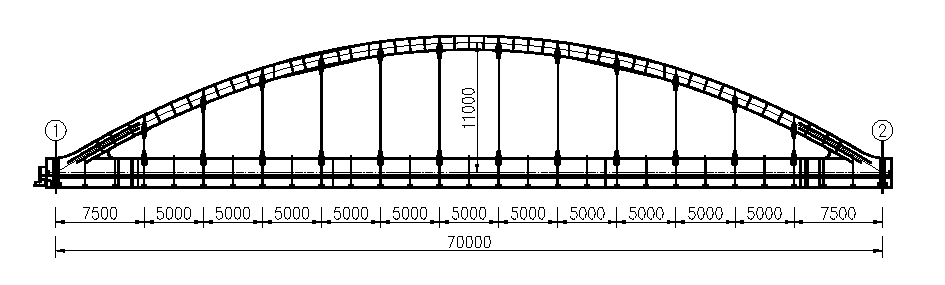
\includegraphics{/WK2/rysunki/widok_z_boku_croped.pdf}} 
	\captionsetup{justification=centering}
	\caption{Widok z boku na konstrukcję stalową dźwigara łukowego wiaduktu WK3}
	\label{fig: wk2_side_view}
\end{figure}

 Przekrój poprzeczny dźwigarów łukowych zaprojektowano jako skrzynkowy (rys. \ref{fig: wk2_cross_sect}). Pomost wykonano jako ortotropowy, z blachy wzmocnionej żebrami podłużnymi i poprzecznicami o przekroju teowym. Poprzecznice rozmieszczono w rozstawie 2.5 m. Ściąg łuku stanowią belki dwuteowe, po jednej dla każdego dźwigara łukowego. Przekrój ściągu zmienia się z dwuteowego na skrzynkowy w strefie podporowej. Na rysunku \ref{fig: wk2_cross_sect_deck} przestawiono przekrój poprzeczny pomostu i ściągu w strefie podporowej. 
  \begin{figure}[h]
 	\centering
 	\subfloat{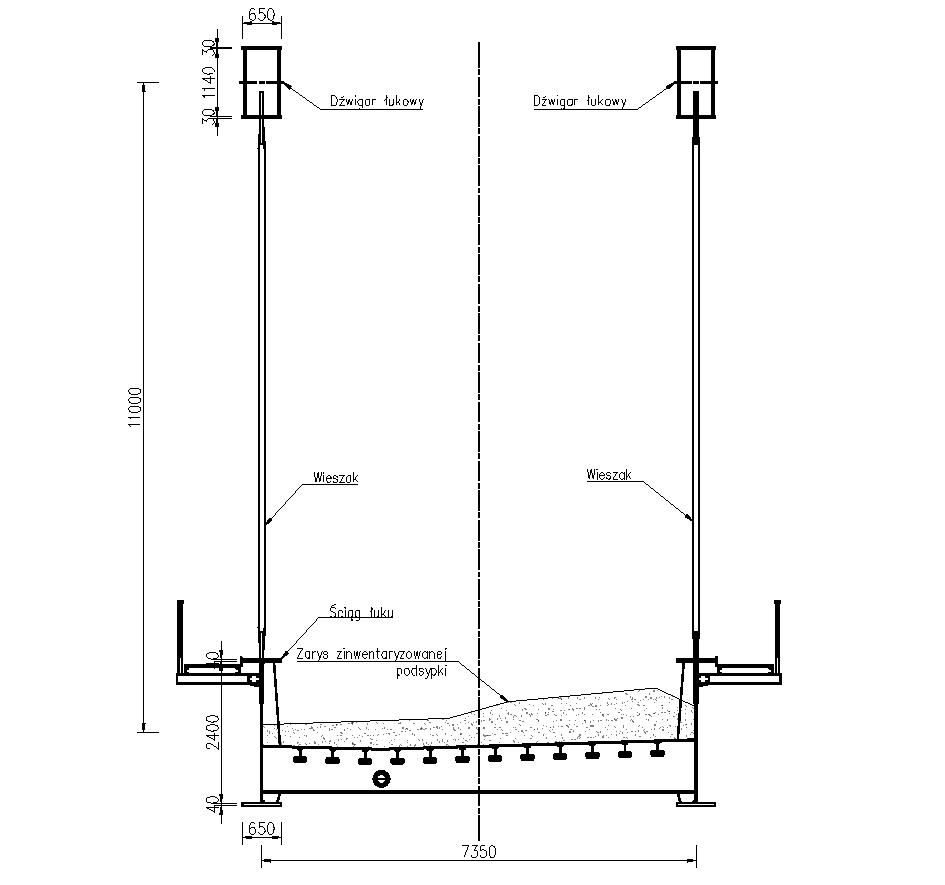
\includegraphics[height=0.6\textheight]{/WK2/rysunki/przekroj_dzwigara_croped.pdf}} 
 	\captionsetup{justification=centering}
 	\caption{Przekrój poprzeczny konstrukcji stalowej wiaduktu WK2 w środku rozpiętości}
 	\label{fig: wk2_cross_sect}
 \end{figure}
 \begin{figure}[h]
 	\centering
 	\subfloat{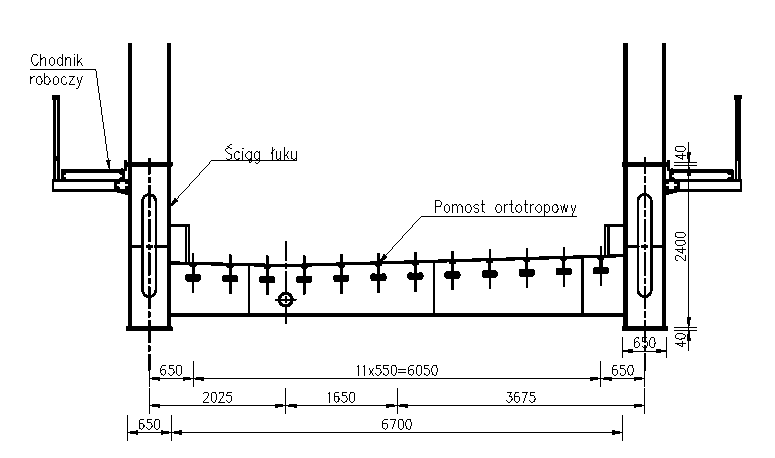
\includegraphics[height=0.25\textheight]{/WK2/rysunki/przekroj_poprzeczny_croped.pdf}} 
 	\captionsetup{justification=centering}
 	\caption{Przekrój poprzeczny przez pomost w strefie podporowej wiaduktu WK2}
 	\label{fig: wk2_cross_sect_deck}
 \end{figure}
 
 W zrealizowanym wariancie pomost został podwieszony do łuku za pomocą prętowych, prostych wieszaków o średnicy 100 mm. Po każdej ze stron zamontowano 12 wieszaków w rozstawie co 5 m. Wieszaki zostały połączone z dźwigarem i ściągiem sztywnym połączeniem spawanym. Rzeczywisty widok zrealizowanego przęsła pokazano na rysunku \ref{fig: wk2_foto_widok_front}, detale konstrukcyjne w obrębie strefy podporowej na rysunku \ref{fig:  wk2_foto_wezglowie}, a połączenie wieszaka ze ściągiem na rysunku \ref{fig: wk2_foto_wieszak}.

\begin{figure}[h]
	\centering
	\subfloat{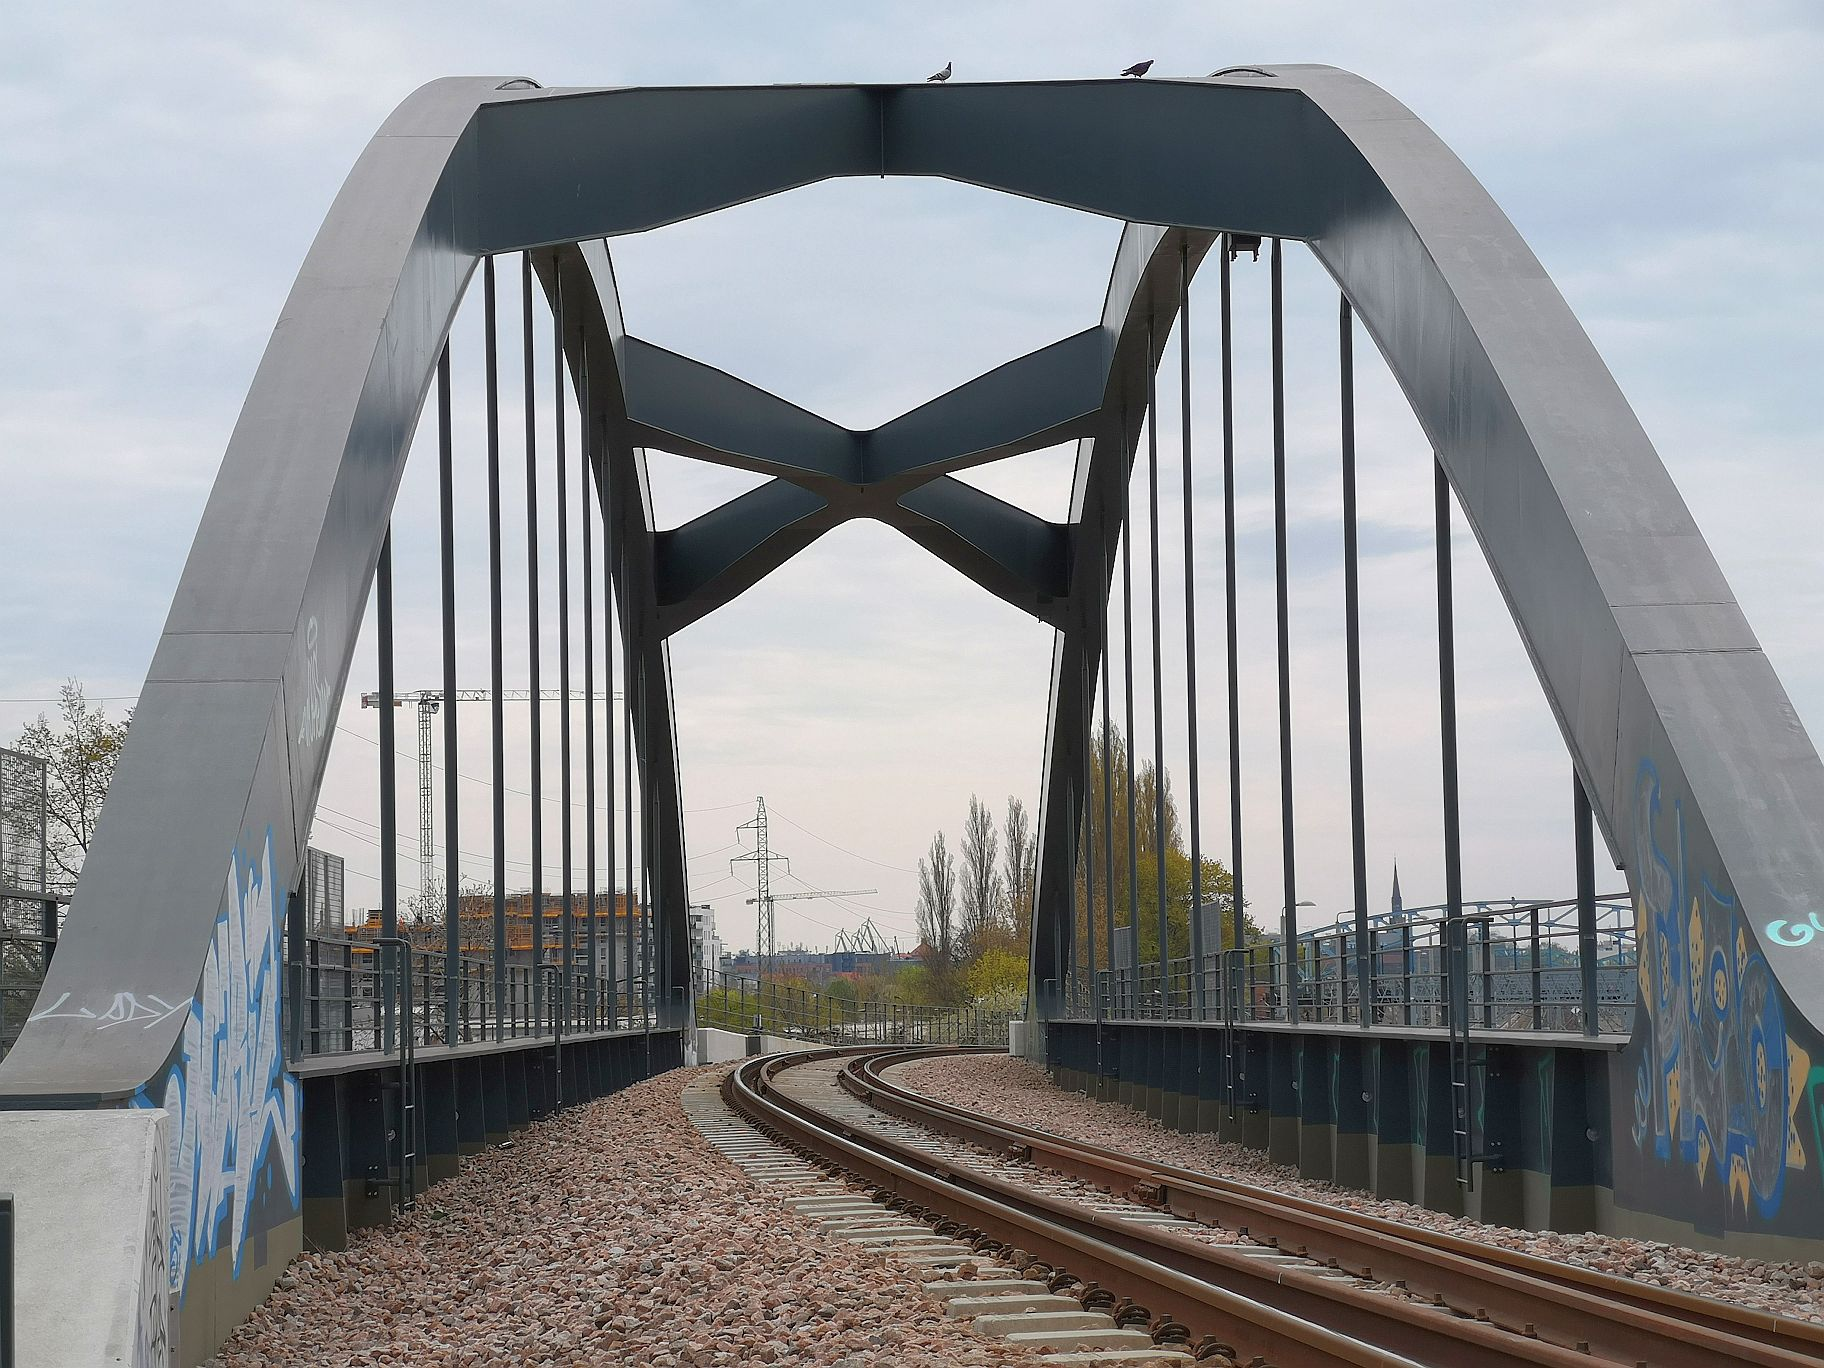
\includegraphics[height=0.35\textheight]{/WK2/zdjecia/widok_front2.jpg}} 
	\captionsetup{justification=centering}
	\caption{Widok od frontu na wiadukt WK2}
	\label{fig: wk2_foto_widok_front}
\end{figure}
\begin{figure}[h]
	\centering
	\subfloat[Widok z góry]{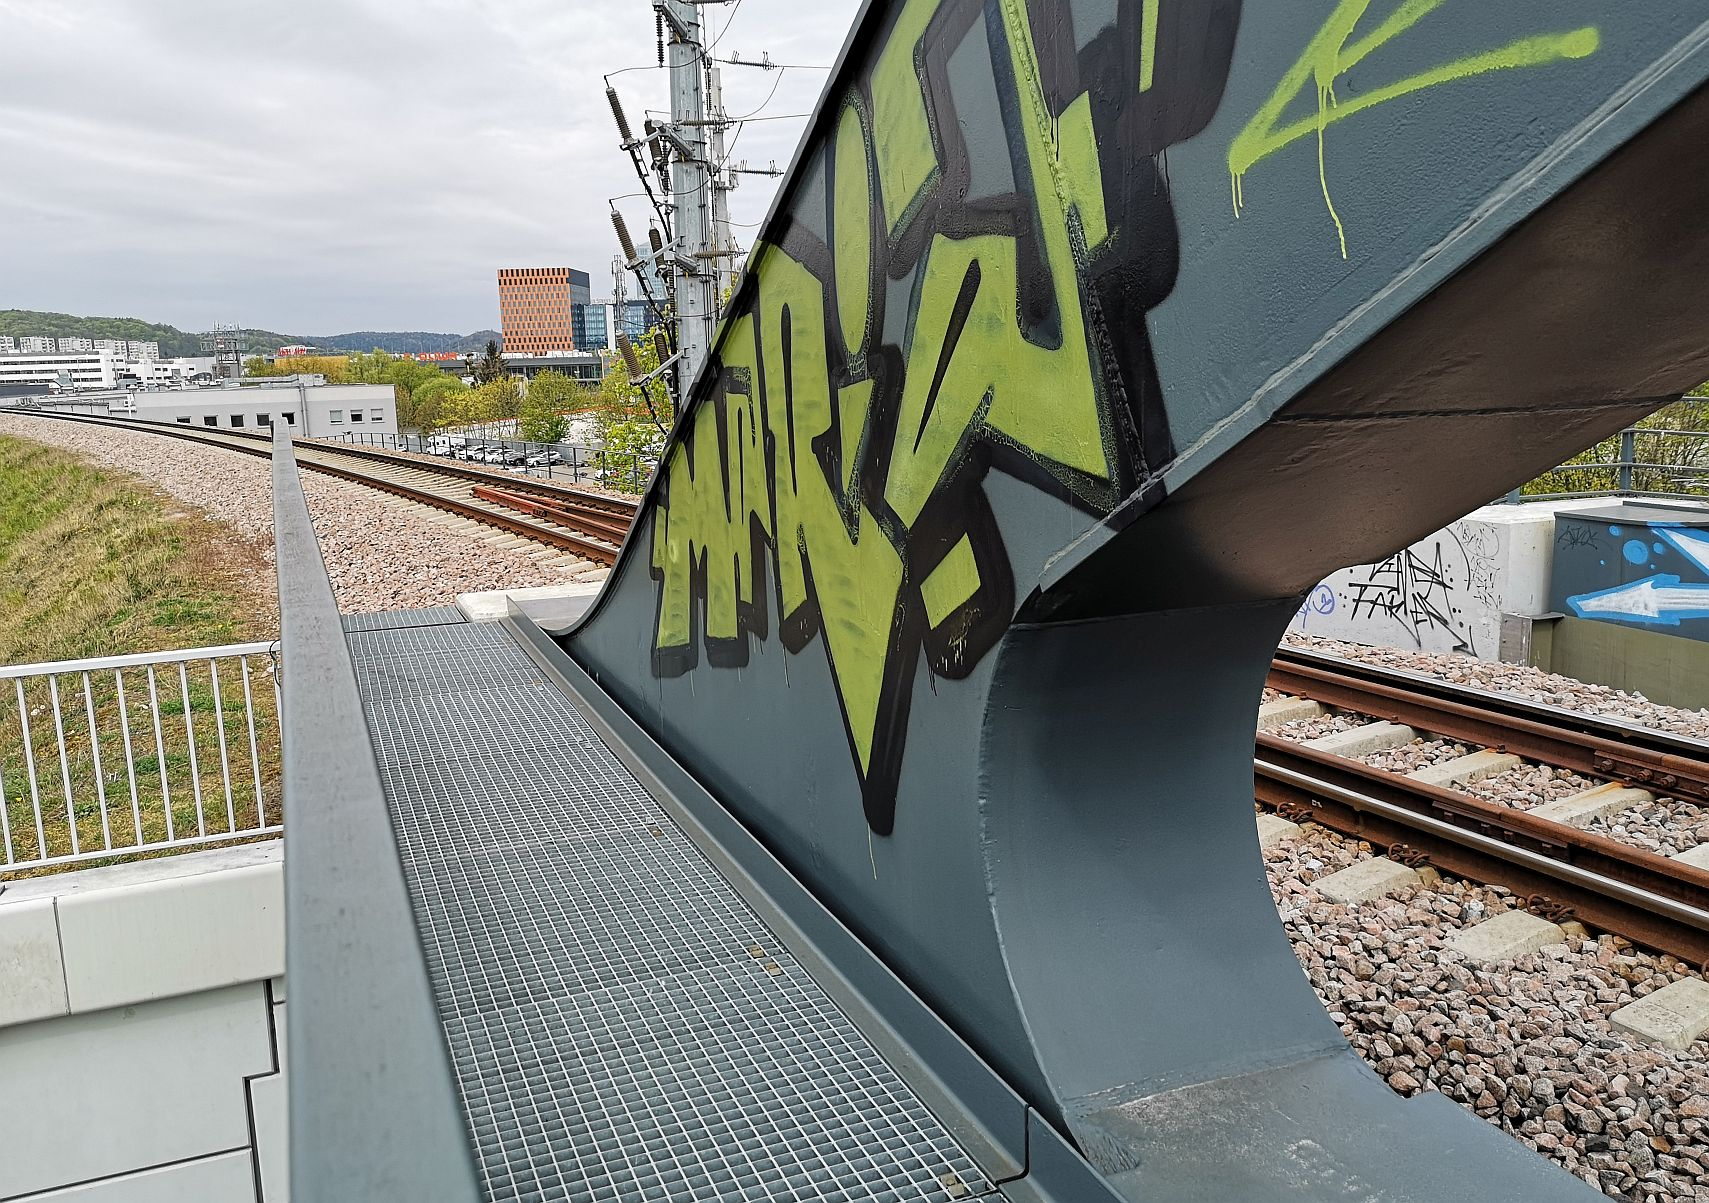
\includegraphics[height=0.2\textheight]{/WK2/zdjecia/wezglowie.jpg}} 
	\qquad
	\subfloat[Widok z dołu]{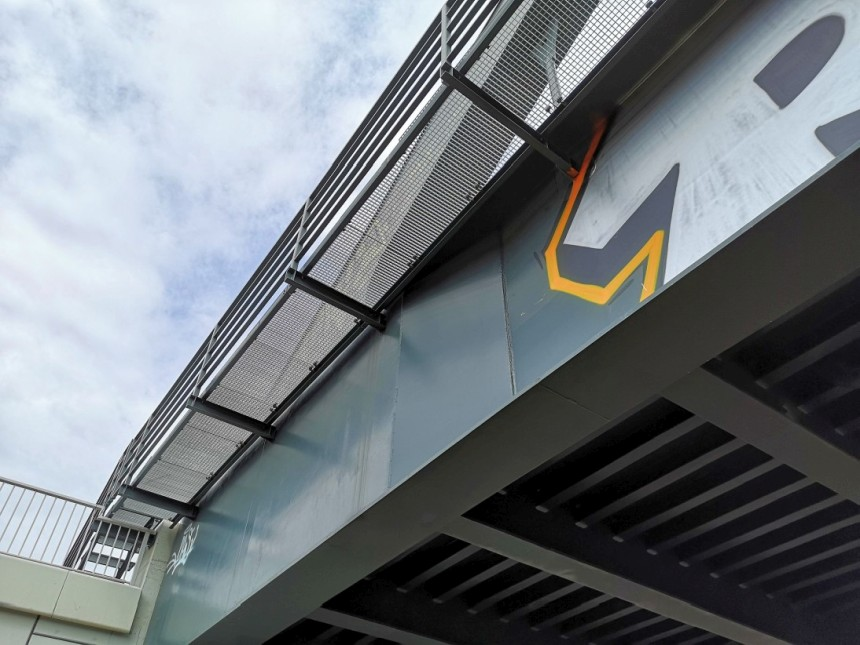
\includegraphics[height=0.2\textheight]{/WK2/zdjecia/detal_wezglowie_dol.jpg}}
	\captionsetup{justification=centering}
	\caption{Szczegóły konstrukcyjne w obrębie połączenia łuku ze ściągiem}
	\label{fig: wk2_foto_wezglowie}
\end{figure}
\begin{figure}[h]
	\centering
	\subfloat{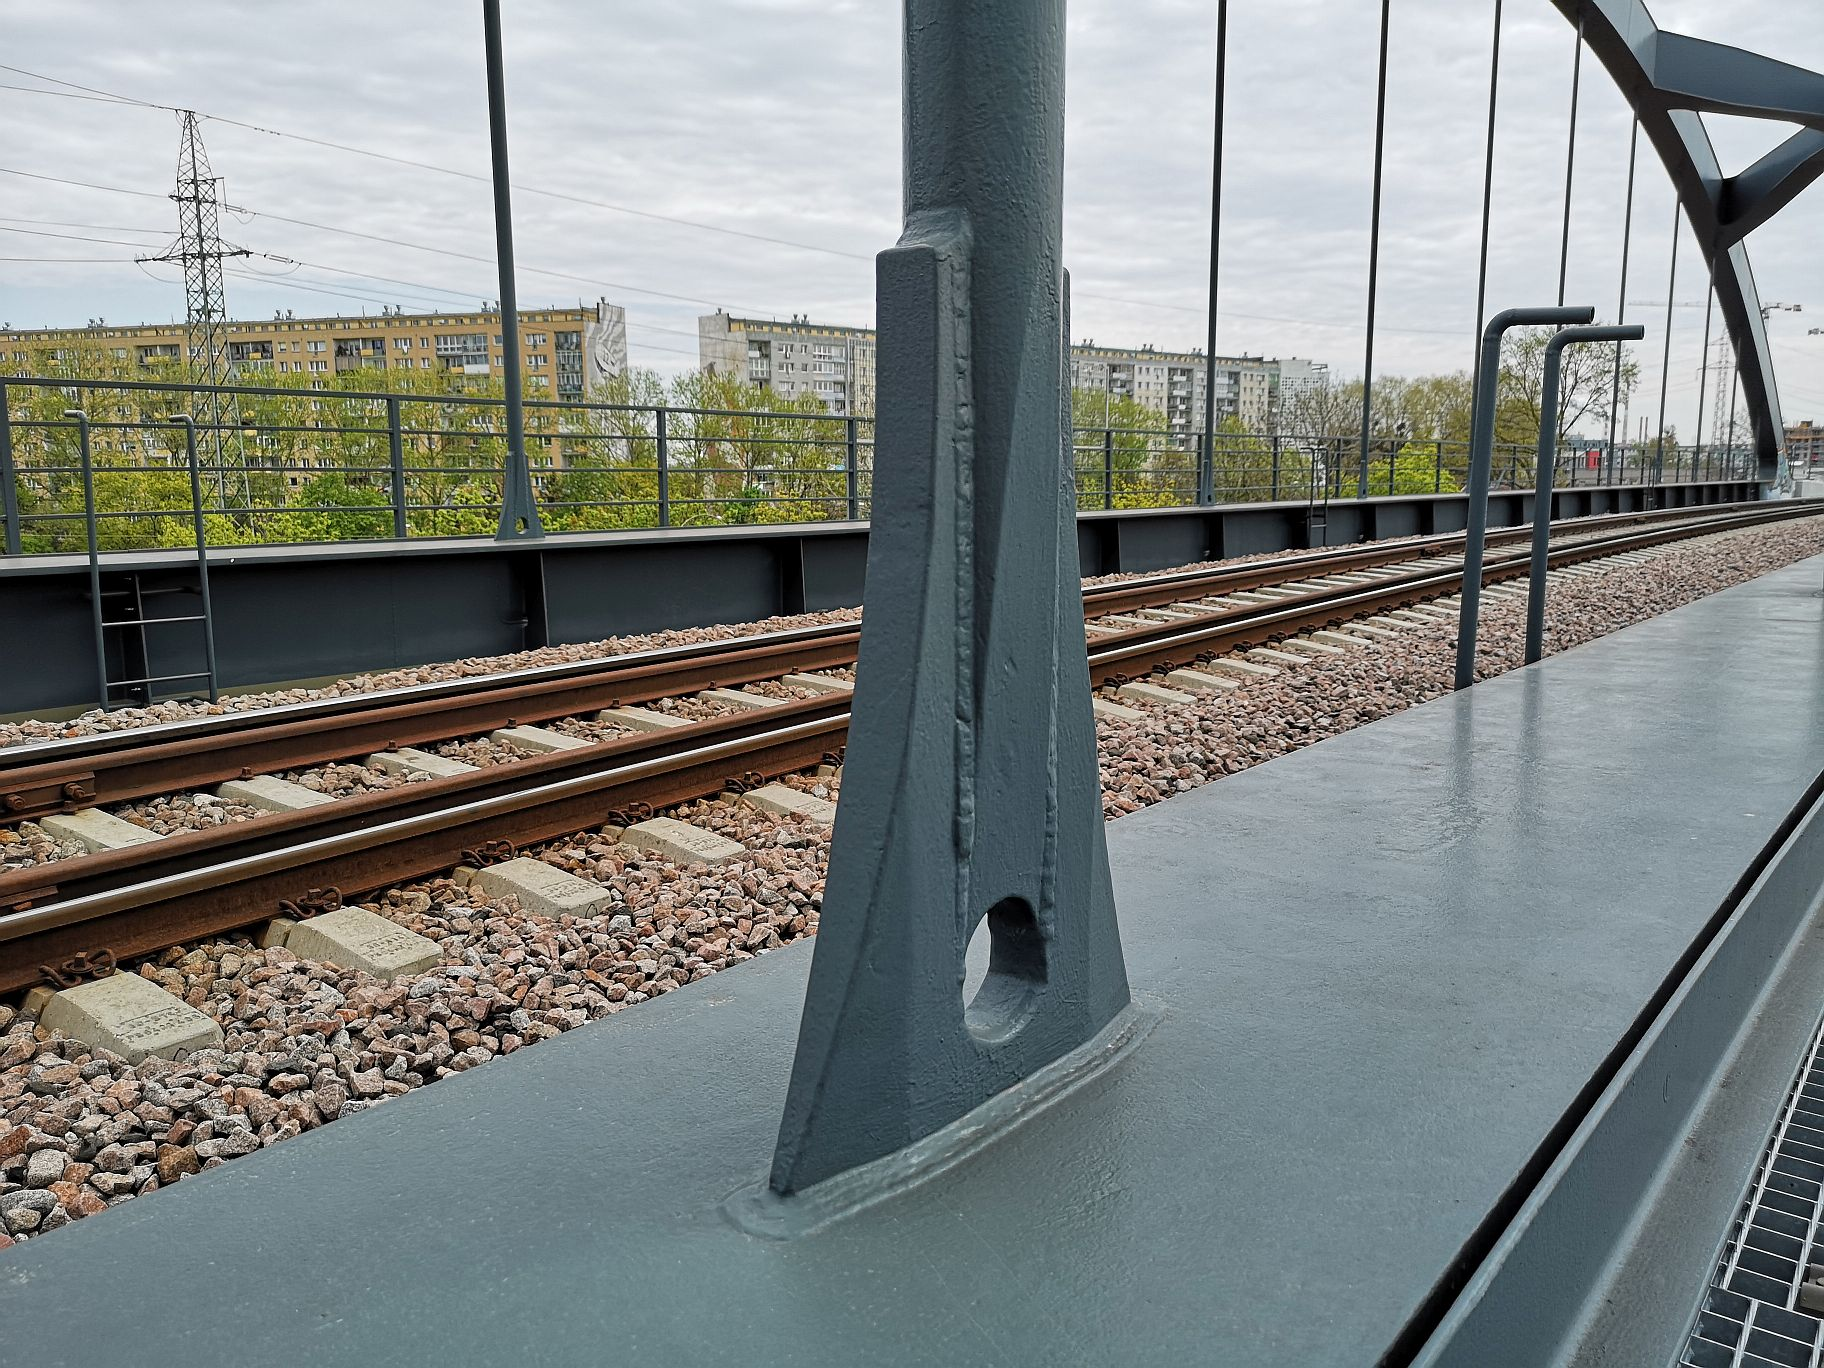
\includegraphics[height=0.2\textheight]{/WK2/zdjecia/zakotwienie_wieszak.jpg}}
	\captionsetup{justification=centering}
	\caption{Detal połączenia wieszaka łuku z pomostem}
	\label{fig: wk2_foto_wieszak}
\end{figure}
Na obiekcie po wybudowaniu przeprowadzono badania odbiorcze. Próbne obciążenia odbyły się w dniu 14.04.2015 i zostały przeprowadzone przez zespół naukowców z Politechniki Śląskiej i Politechniki Gdańskiej \parencite{azinski2015}. Wykonano badania statyczne i dynamiczne. Wyniki jednych i drugich pomiarów posłużą jako elementy kalibracji modelu lub spełnią rolę punktu odniesienia dla wyników badań zrealizowanych w ramach tej pracy. W ramach pomiarów statycznych zrealizowano dwa interesujące, z punktu widzenia tej pracy, ustawienia obciążenia. Ustawienie U1 z obciążeniem zorientowanym symetrycznie na obiekcie oraz ustawienie U2 z obciążeniem wywołującym maksymalne ugięcia w $1/4$ rozpiętości przęsła. Pomiary przemieszczeń wykonywano w 6 punktach zlokalizowanych w $1/4$, $1/2$ i $3/4$ rozpiętości przęsła, po obu jego stronach. Czujniki zamocowano do konstrukcji w osiach ściągów, na dolnych lub górnych pasach. Obciążenie statyczne stanowiły dwie lokomotywy spalinowe typu: SM-48 i BR232. Pomierzone ugięcia statyczne zostaną użyte jako dodatkowe kyterium kalibracji modelu numerycznego.
W ramach badań dynamicznych mierzono przyspieszenia konstrukcji po wymuszeniu obciążeniem impulsowym. Impuls generowano przez upadek jednej osi koparki dwudrogowej i zeskoków drezyny z progu. Na postawie przebiegów drgań swobodnych zidentyfikowano częstotliwości drgań własnych przęsła i towarzyszące im tłumienia. Do identyfikacji użyto algorytmu ERA. Zidentyfikowane częstotliwości drgań i tłumienia przęsła posłużą do porównania z wynikami badań przeprowadzonymi w ramach tej pracy.


\section{Budowa modelu numerycznego}

Na potrzeby analiz numerycznych zbudowano model MES w środowisku SOFiSTiK (rys. \ref{fig: model_wk2_visualization}) Model przestrzenny składa się kilku rodzajów elementów skończonych. Z jednowymiarowych elementów belkowych wykonano łuki, stężenia, belki ściągu, wzmocnienia wezgłowii i żebra pomostu ortotropowego. Z elementów kratowych stworzono wieszaki. Blachę pomostu wykonano z czterowęzłowych elementów powłokowych. Połączenia pomiędzy końcami wieszaków i osiami łuku oraz ściągu zrealizowano przez połączenia kinematyczne translacji i rotacji węzłów. Podparcia pionowe w miejscach łożysk mostu zrealizowano za pomocą sztywnych więzów węzłów. Nie zablokowano przesuwów podłużnych i poprzecznych za pomocą blokady przemieszczeń. Zamiast tego na obu kierunkach zamocowano elastyczne elementy o bardzo dużej sztywności. Dostosowanie do istniejących warunków łożyskowania opisane zostało w dalszej części rozdziału. Usztywnienia wezgłowii zamodelowano za pomocą rusztu elementów belkowych o przekroju składającym się z dwóch blach odsuniętych od siebie na szerokość przekroju skrzynkowego łuku. Elementy strukturalne konstrukcji (takie jak ściągi, pomost, dźwigary łukowe, elementy podparcia itd.) podzielono w modelu na grupy pozwalające odnosić się do nich jako całości. Przekroje elementów belkowych przyjęto zgodnie z dostępną dokumentacją (!!!). Wymiary przekrojów zmiennych po długości zostały interpolowane liniowo. Widoczne na rysunku (\ref{fig: model_wk2_static_scheme}) dodatkowe połączenia kinematyczne są przygotowaniem dla możliwości podłączenia innych konfiguracji wieszaków.



\begin{figure}[h]
	\centering
	\subfloat[Widok A]{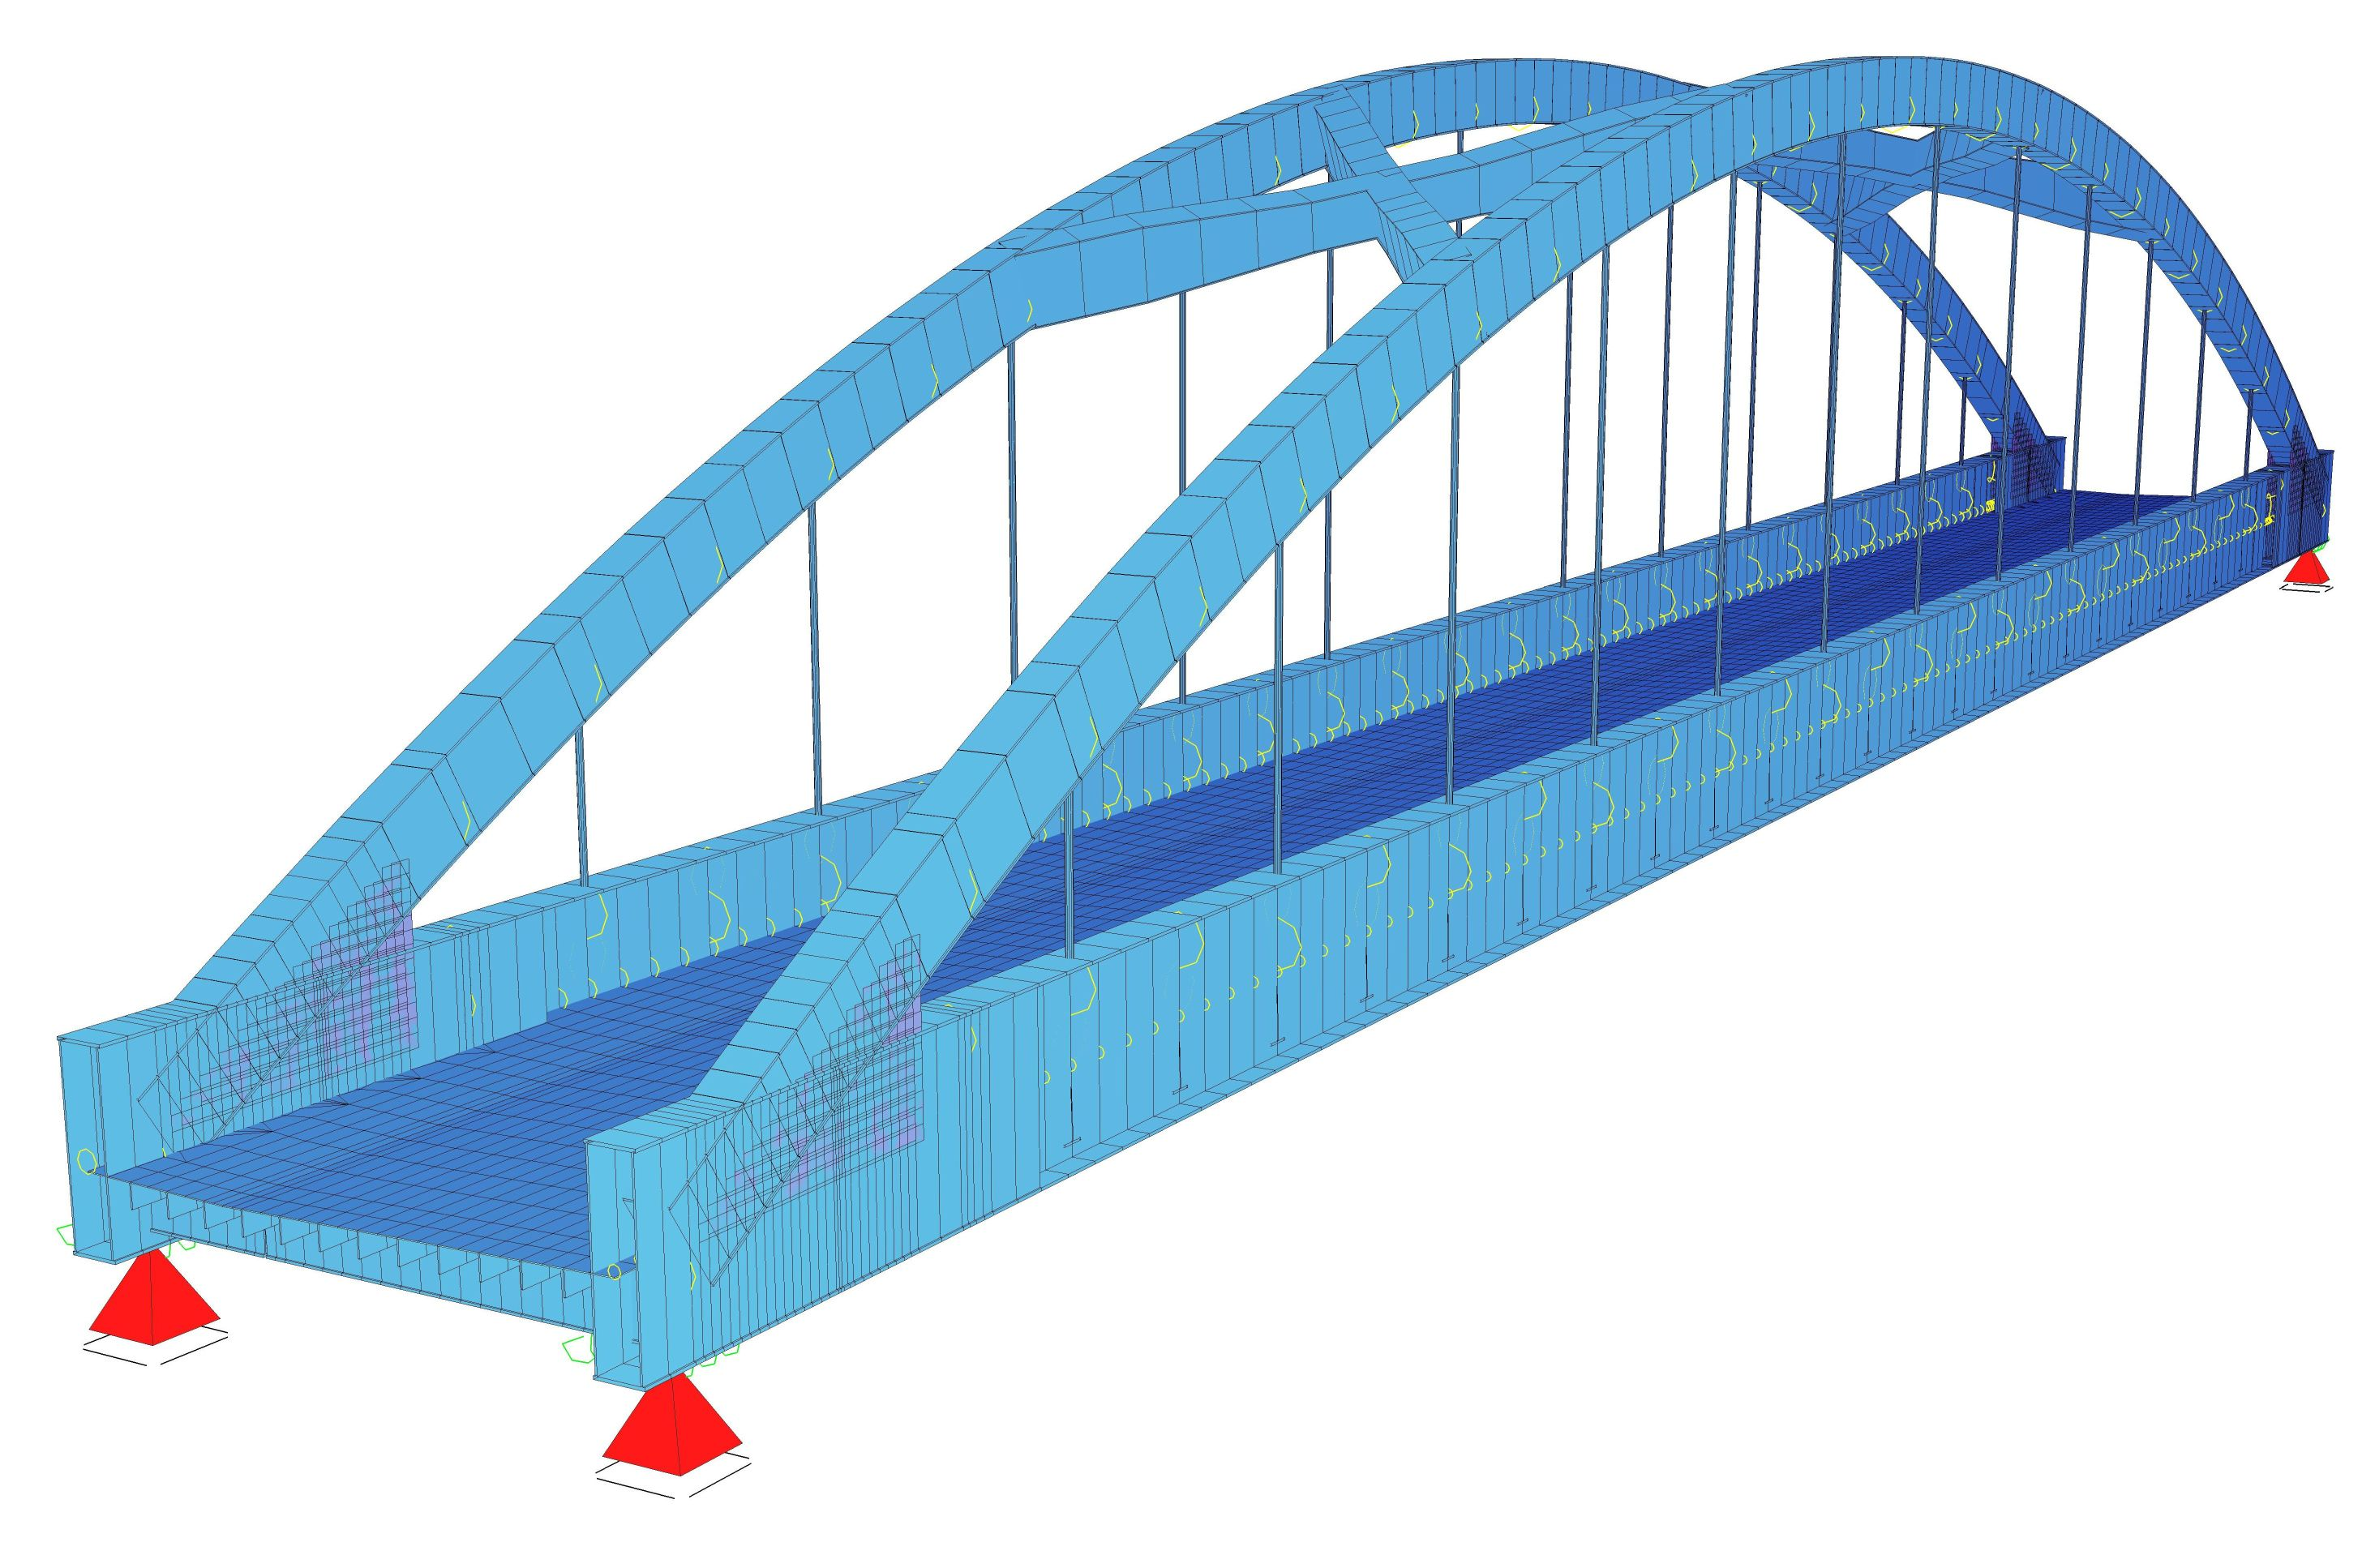
\includegraphics[width=0.5\linewidth]{/WK2/model/SCIAG_PAR_v01_vis_1.jpg}}%
	\subfloat[Widok B]{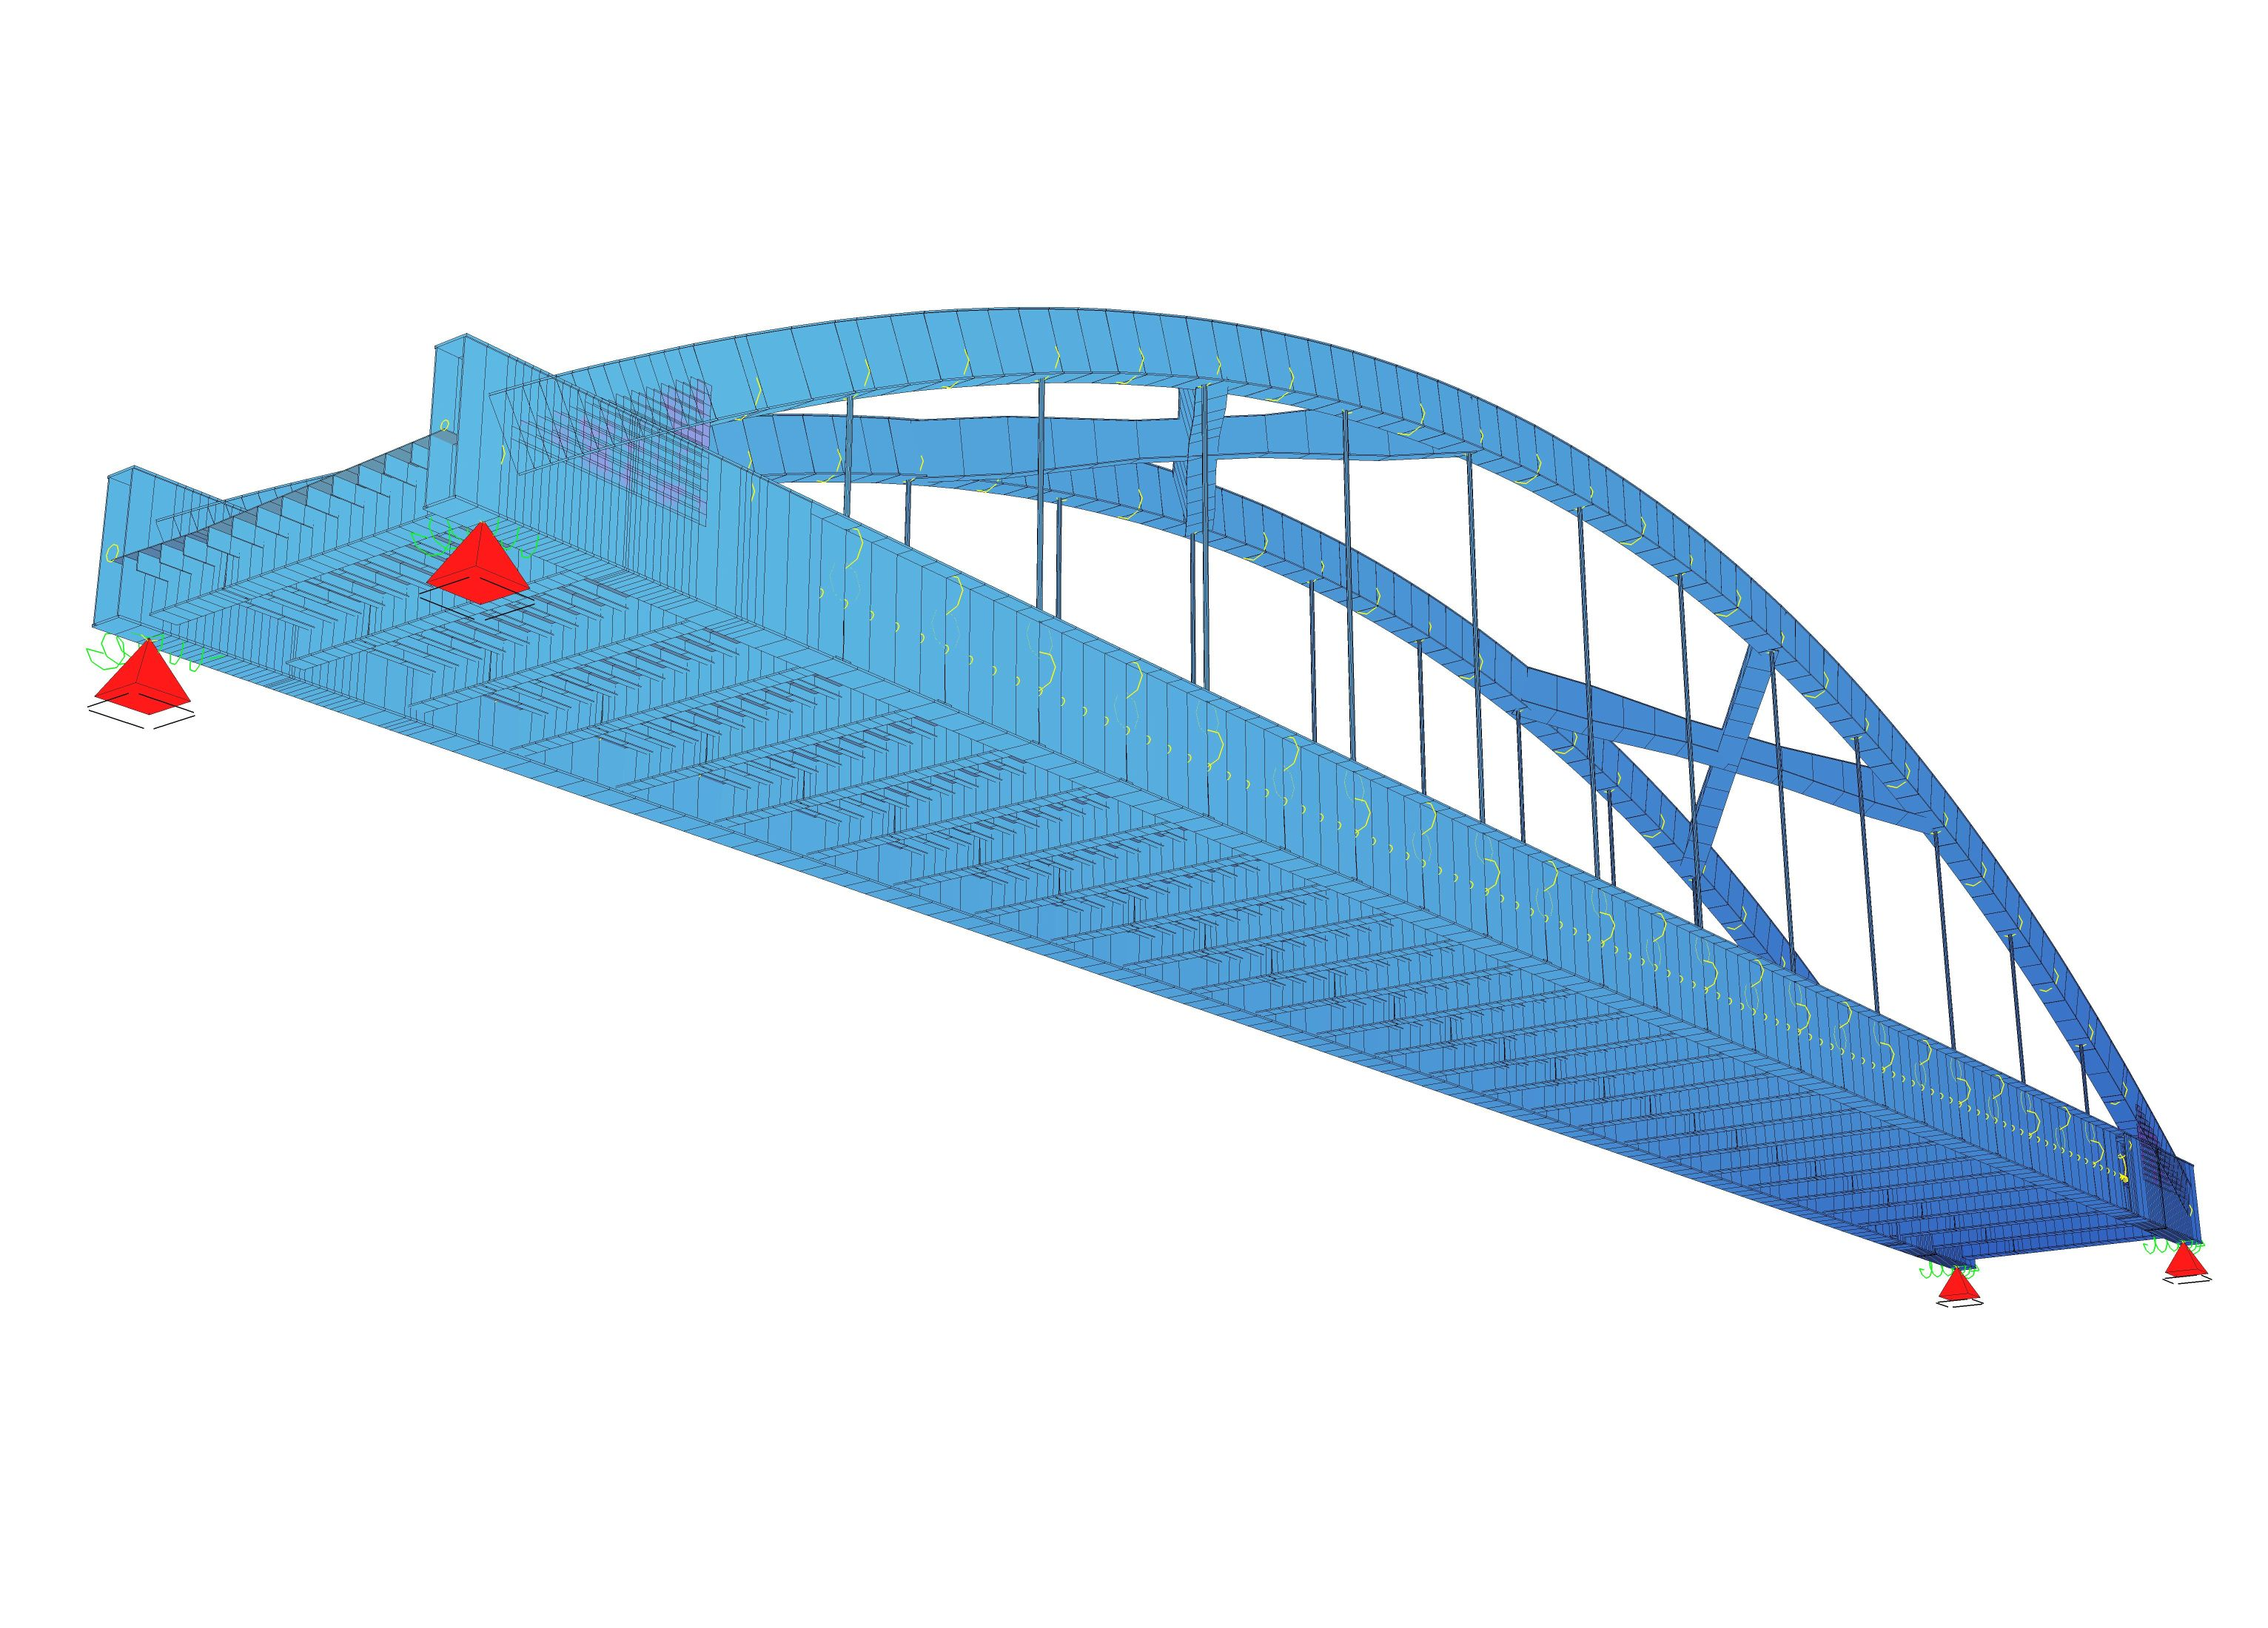
\includegraphics[width=0.5\linewidth]{/WK2/model/SCIAG_PAR_v01_vis_2.jpg}}
	\captionsetup{justification=centering}
	\caption{PODMIENIC NA RZECZYWISTE WYMIARY KONSTRUKCJI!!!!! Wizualizacja przestrzennego modelu numerycznego wiaduktu WK2 Pomorskiej Kolei Metropolitalnej}
	\label{fig: model_wk2_visualization}
	
\end{figure}
\begin{figure}[h]
	\centering
	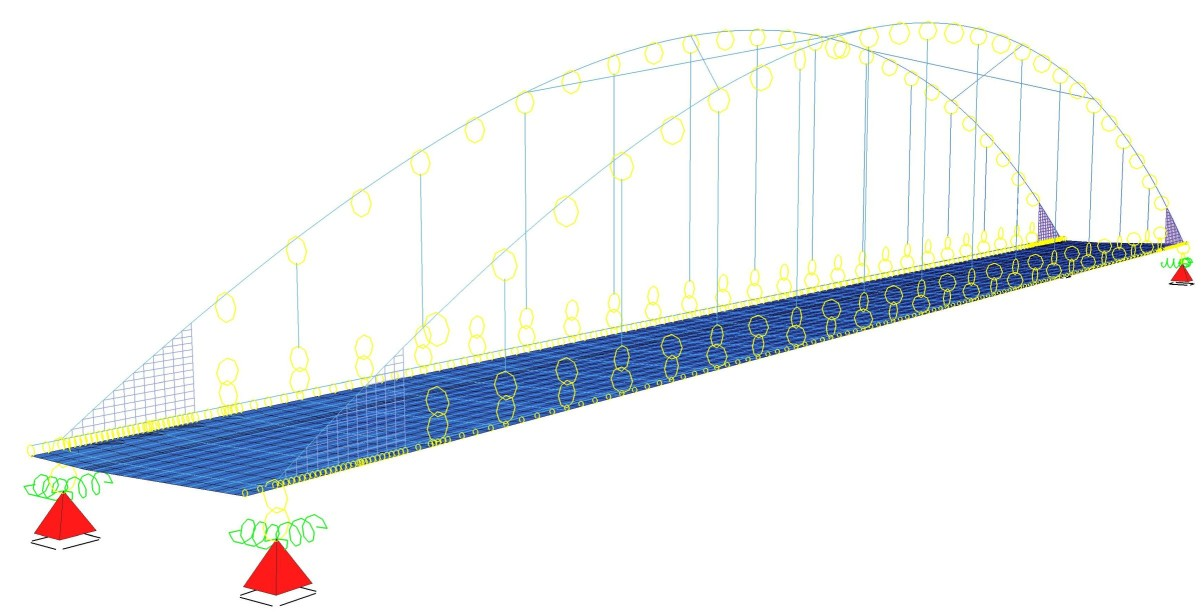
\includegraphics[width=0.8\linewidth]{/WK2/model/SCIAG_PAR_v01_schemat_1.jpg}
	\captionsetup{justification=centering}
	\caption{Schemat statyczny modelu numerycznego wiaduktu WK2 Pomorskiej Kolei Metropolitalnej}
	\label{fig: model_wk2_static_scheme}
\end{figure}

Obciążenie ciężarem własnym konstrukcji zostało wygenerowane na podstawie ciężarów wprowadzonych przekrojów elementów liniowych bądź grubości elementów powłokowych. Dodatkowe elementy takie jak przepony i zakotwienia wieszaków dodane zostały jako obciążenia węzłowe. Osobny przypadek obciążenia stanowi pomost roboczy dodany jako ekwiwalentne obciążenie węzłowe i momenty zginające. Ostatnim obciążeniem stałym jest ciężar tłucznia. Z uwagi na ułożenie toru po łuku w planie, rozkład tłucznia na obiekcie nie jest regularną, symetryczną bryłą. Dostępna dokumentacja obiektu nie dostarcza dokładnych informacji o ułożeniu podsypki na pomoście. Podsypka została w prosty sposób zinwentaryzowana przez pomiar grubości w niektórych punktach charakterystycznych. Na rysunku \ref{fig: wk2_cross_sect} zaprezentowano zinwentaryzowany układ tłucznia w przekroju przęsłowym. Zastosowana metoda pomiaru objętości tłucznia nie jest dokładna i na pewno nie odzwierciedla realnego rozkładu ciężaru podsypki na obiekcie. Z tego względu podzielono obciążenie tłuczniem na dwa osobne przypadki: równomiernie rozłożone obciążenie na całym pomoście i obciążenie równomierne o szerokości (!!!) usytuowane wzdłuż osi toru. Wartość obciążenia tłuczniem przyjęto z normy (!!!).



\section{Badania - identyfikacja modalna: wybór punktów, opis badań, wyniki identyfikacji}
Przed przystąpieniem do procesu optymalizacji układu statycznego dźwigara łukowego model należało skalibrować. Z uwagi na zakres planowanych analiz kluczowe dla analizy dynamicznej jest aby model w odpowiedni sposób odzwierciedlał rzeczywistość w zakresie parametrów modalnych. Mając do dyspozycji rzeczywisty obiekt, zdecydowano o wykonaniu badań terenowych, które pozwolą na identyfikację częstotliwości i postaci drgań własnych oraz towarzyszącego im tłumienia. Obiekt jest w ciągłej eksploatacji. Z tych względów zdecydowano o wykorzystaniu Operacyjnej Analizy Modalnej do identyfikacji parametrów modalnych przęsła.
Przed przystąpieniem do badań przygotowano plan zawierający kluczowe punkty, bez których spełnienia badania mogą zakończyć się niepowodzeniem lub wyniki mogą być trudne w interpretacji. \cite{Brincker2015} sporządzili listę zaleceń, które należy wypełnić w trakcie przygotowań eksperymentu OMA aby zakończył się on powodzeniem. Podobne zalecenia w swojej pracy sformułował \cite{Poprawa2018}. W kontekście założonych celów i wybranego obiektu badawczego główne z nich to:
\begin{itemize}
\item opracowanie strategi prowadzenia badań i akwizycji danych,
\item uzgodnienia administracyjne - wstęp na obiekt i możliwość prowadzenia badań pod ruchem,
\item dobranie sprzętu pomiarowego.
\end{itemize}

Zarządca obiektu zezwolił na prowadzenie badań pod ruchem w towarzystwie sygnalisty. Średnie natężenie ruchu na obiekcie w trakcie badań to około 1 przejazd na 30 min. Wybór sprzętu pomiarowego ograniczał się do zastosowania posiadanego sprzętu do akwizycji przyspieszeń opisanego w punkcie (!!!). Najistotniejszym punktem przygotowania badań było opracowanie strategii badań. Według \cite{Brincker2015} plan badań OMA powinien zawierać następujące punkty:
\begin{itemize}
	\item sporządzoną siatkę pomiarową,
	\item kolejność ustawień czujników w seriach pomiarowych,
	\item określenie liczby osób potrzebnych do przeprowadzenia eksperymentu,
	\item zapewnienie bezpieczeństwa w trakcie badań,
	\item określenie parametrów akwizycji danych (częstotliwość próbkowania, długość pomiarów, liczba powtórzeń serii pomiarowych itd.)
\end{itemize}

Dostępny system pomiarowy składał się z dwóch akcelerometrów 3-osiowych i z dwóch czujników 1-osiowych.  Mając do dyspozycji ograniczoną liczbę jednocześnie mierzonych punktów należało przeprowadzić symulację najlepszego rozmieszczenia punktów pomiarowych na obiekcie. Przykłady metod pozwalających na optymalne rozmieszczenie punktów pomiarowych w analizach dynamicznych zaprezentowano w literaturze i najczęściej opierają się one na wyznaczeniu reprezentatywnego wskaźnika, dzięki któremu da się porównać różne ustawienia. Między innymi \cite{Kammer1991,Papadopoulos1998} zaproponowali użycie Modalnej Energii Kinetycznej \teng{Modal Kinetic Energy}, \cite{Udwadia1994} macierzy informacyjnej Fishera \teng{Fisher Information Matrix}, a \cite{Penny1994,Allemang2003} macierzy MAC dla zestawu modów. \cite{Zhang2017} przedstawili zwięzłe zestawienie powyższych metod i zaproponowali opcję optymalizującą lokalizację punktów pomiarowych przy wielu ustawieniach pomiarowych, zarówno dla punktów pomiarowych jak i punktów referencyjnych. Autorzy zwracają również uwagę, że przy wielu punktach pomiaru ścisła ocena wszystkich możliwych ustawień jest wymagająca obliczeniowo bądź niemożliwa. Z tego względu stosowane są algorytmy heurystyczne bądź meta-heurystyczne. W poniższej pracy wykorzystano metodę wykorzystującą kryterium MAC. Podobne postępowanie przedstawił w swojej pracy \cite{Poprawa2018}. Polega ono na wyznaczeniu teoretycznych postaci drgań własnych na przykład z dostępnego modelu MES. Dla zbioru możliwych położeń czujników odczytywane są przemieszczenia znormalizowane danej postaci drgań. Ze zbioru możliwych położeń wybierane są punkty, gdzie umieszczone mają zostać czujniki. Następne odczytywane są dla nich przemieszczenia znormalizowane (z analizy modalnej) dla wszystkich interesujących modów. Posiłkując się opisem postaci drgań w wybranych punktach tworzona jest macierz współczynników MAC. Każdą postać porównuje się ze wszystkimi innymi i najczęściej z samą sobą. W ten sposób na przekątnej macierzy pojawiają się wartości równe 1 - idealne dopasowanie według kryterium MAC - co dla identycznych wektorów jest oczywiste. Poza przekątną wartości MAC mieszczą się między 0, a 1. Celem analizy jest, aby poza przekątną wartości były możliwie małe. Przy małym dopasowaniu, zidentyfikowane postaci będą miały szanse być zidentyfikowane jednoznacznie przy mocno ograniczonej liczbie punktów pomiarowych i bliskim położeniu modów w dziedzinie częstotliwości.


\begin{figure}[h]
	\centering
	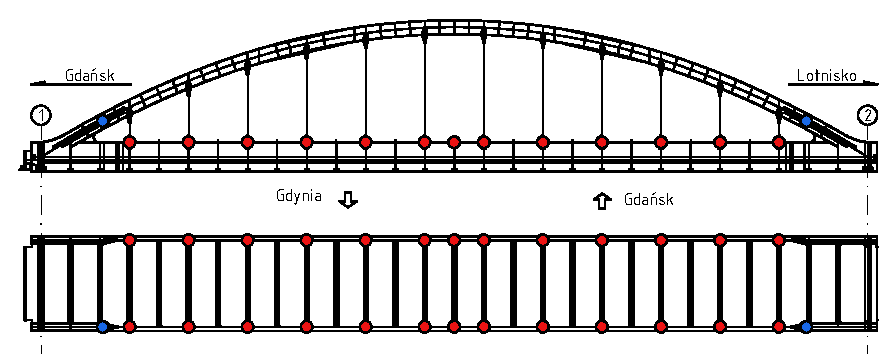
\includegraphics{/WK2/rysunki/punkty_pomiarowe_automac_croped.pdf}
	\captionsetup{justification=centering}
	\caption{}
	\label{fig: wk2_automac_points_all}
\end{figure}




Zastosowane kryteria: max mac 0.6, rowno na obie strony, maksymalna srednia z wektorow punktow. Dodac zmiennosc w kombinacjach maksymalnego momentu jako przestroge.


\begin{figure}[h]
	\centering
	\subfloat[System akwizycji danych: komputer i wzmacniacz pomiarowy HBM PMX]{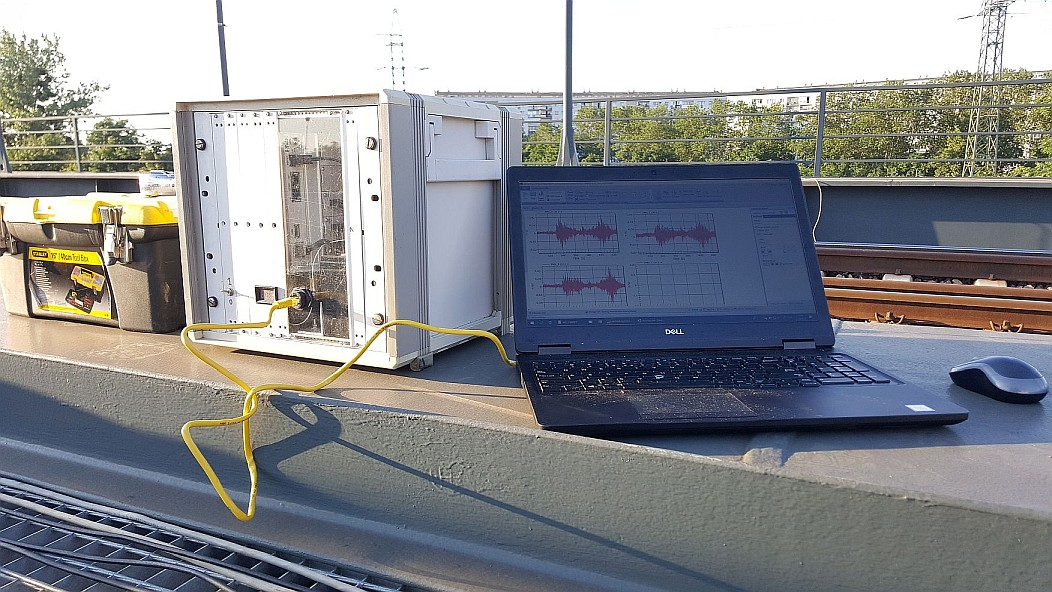
\includegraphics[width=0.48\linewidth]{/WK2/zdjecia/system_pomiarowy.jpg}} \quad 
	\subfloat[3 osiowy akcelerometr piezorezystancyjny]{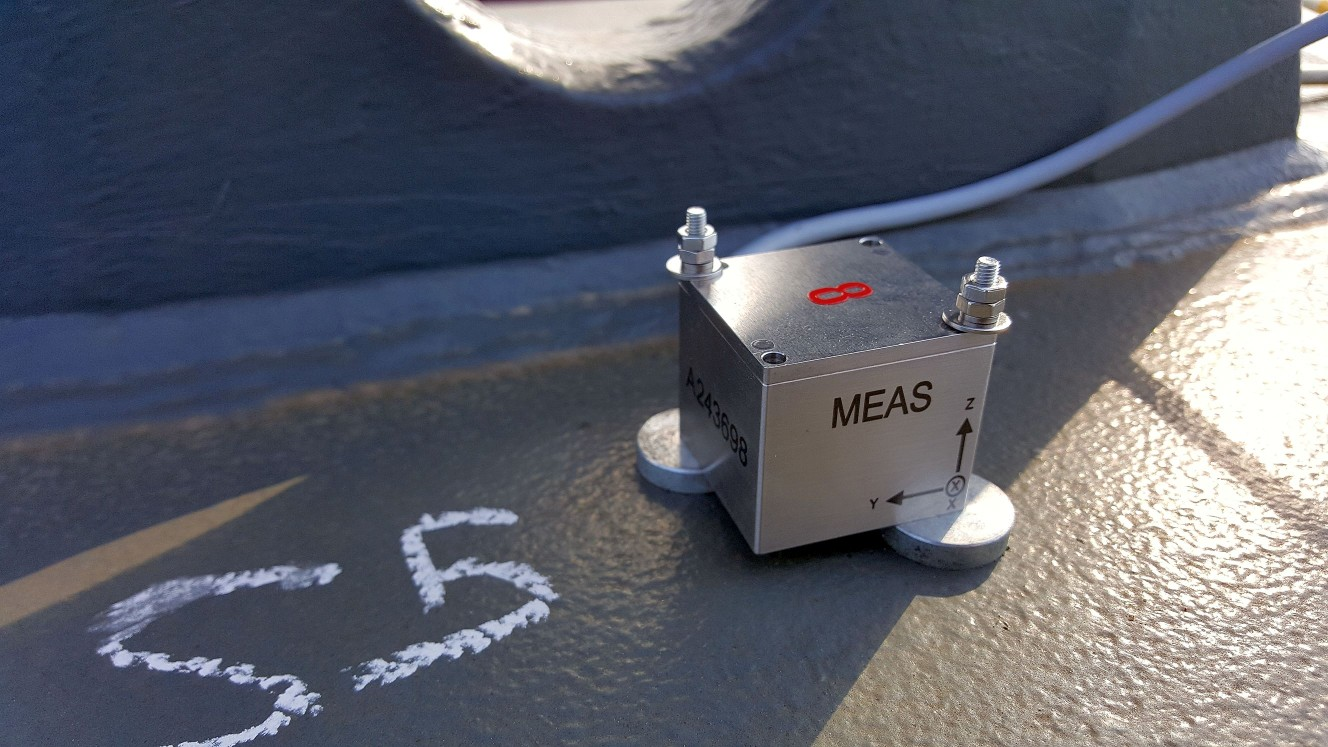
\includegraphics[width=0.48\linewidth]{/WK2/zdjecia/czujnik_3_osie.jpg}} 
	\captionsetup{justification=centering}
	\caption{System pomiarowy użyty do identyfikacji modalnej wiaduktu WK2}
	\label{fig: wk2_foto_aparatura}
\end{figure}



\begin{figure}[h]
	\centering
	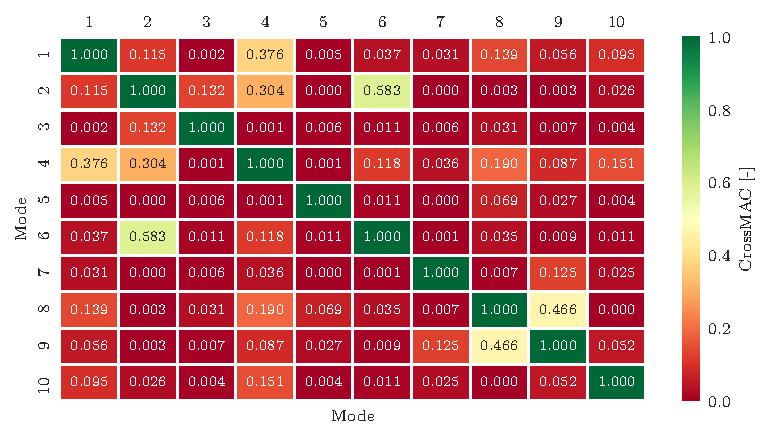
\includegraphics[width=\textwidth]{WK2/correlogram_badania.pdf}
	\captionsetup{justification=centering}
	\caption{Diagram AUTOMAC dla pierwszych dziesięciu wektorów postaci drgań własnych, odczytanych z modelu dla wybranych punktów pomiarowych}
\end{figure}
\begin{figure}[h]
	\centering
	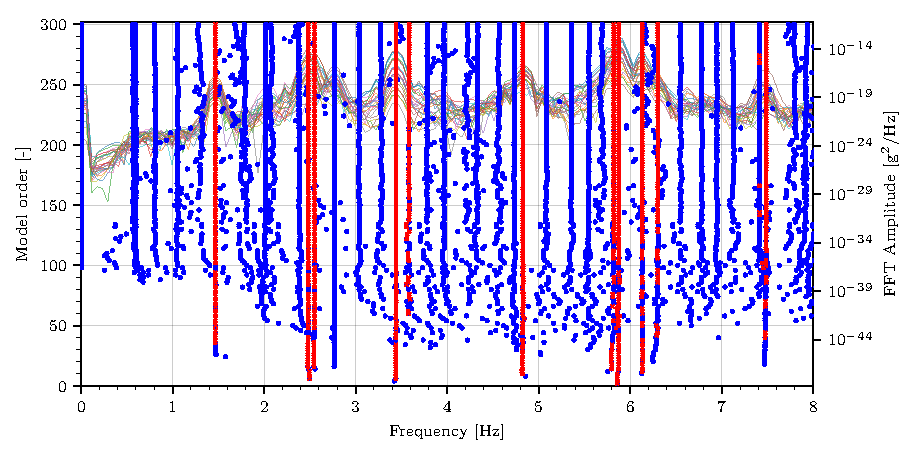
\includegraphics[width=\textwidth]{WK2/diagram_non_filtered.pdf}
	\captionsetup{justification=centering}
	\caption{Diagram stabilizacyjny metody NExT-ERA.}
\end{figure}
\begin{figure}[h]
	\centering
	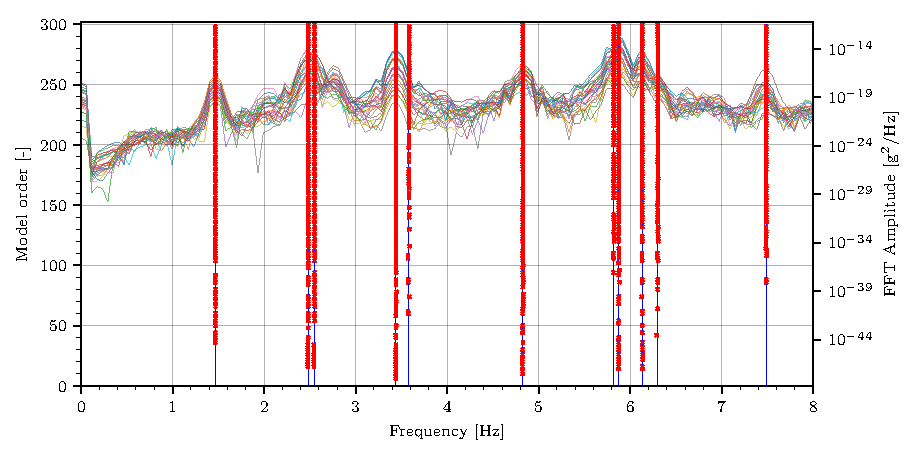
\includegraphics[]{WK2/diagram_filtered2.pdf}
	\captionsetup{justification=centering}
	\caption{Diagram stabilizacyjny metody NExT-ERA.}
\end{figure}
\begin{figure}[h]
	\centering
	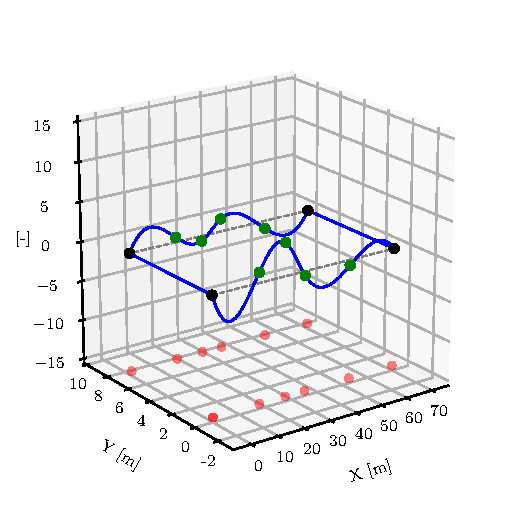
\includegraphics[]{WK2/identified_mode_1.pdf}
	\captionsetup{justification=centering}
	\caption{Diagram stabilizacyjny metody NExT-ERA.}
\end{figure}

\section{Kalibracja modelu numerycznego z wykorzystaniem PSO}
\section{Wielokryterialna optymalizacja modelu: opis + wyniki}
\chapter{Podsumowanie i wnioski}
Podsumowania wnioski










Some claim \parencite{szafranski_oddzialywania_2013,rucka_dynamika_2014}
Parametry metody NeXT-ERA: \parencite{caicedo_practical_2011}
1)	Długość okna użytego przy transformacie Fouriera
2)	Wybór kanału referencyjnego
3)	Wielkość macierzy Hankela – alfa i beta
4)	Liczba biegunów do identyfikacji
5)	Długość i częstotliwość próbkowania sygnału wejściowego

Wykres dwóch pierwszych momentów sygnału – średniej i odchylenie standardowe. Wskazówka do określenia stacjonarności – jeśli wartości są prawie stałe. \parencite{caicedo_practical_2011,bendat_random_2011}


Wybór sygnałów: parametry częstotliwość próbkowania, noise-to-signal ratio i stacjonarność


Blisko położone piki – zmniejszenie częstotliwości próbkowania \parencite{caicedo_practical_2011}


Częstotliwość próbkowania – obniżenie – wartość ok 2 razy większa niż interesujące częstotliwości \parencite{caicedo_practical_2011}


Liczba punktów funkcji kros korelacji jest równa liczbie punktów użytych w FFT, a częstotliwość próbkowania jest równa częstotliwości użytych sygnałów \parencite{caicedo_practical_2011}

MAC kryterium doboru punktów pomiarowych dla testów dynamicznych 


Metoda Welcha \parencite{welch_use_1967}


Oś pionowa oznaczona jako $g^2$ \parencite{caicedo_practical_2011}

Alfa i beta – numer column 4x liczba modów (2x liczba biegunów). Numer wierszy – numer punktów w cross spectral density? \parencite{caicedo_practical_2011}. Ostatecznie chodzi o to by uwzględnić tyle danych z CCF żeby nie ująć ani za dużo ani za mało.


Algorytm filtrowanego diagramu stabilizacyjnego  \parencite{caicedo_practical_2011}

Parametry alfa i beta \parencite{brownjohn_ambient_2010,caicedo_practical_2011,hollkamp_modal_2001,nayeri_study_2009,siringoringo_system_2008,szafranski_oddzialywania_2013}  przyjmować tak żeby alfa zawierała ok dwukrotność liczby biegunów (4x liczba modów) a parametr beta swoim zakresem obejmował odpowiednią liczbę sygnałów)


\printbibliography
\end{document}

